%% $Id: manual.tex,v 1.20 2017/11/22 13:51:40 filipi Exp $
\documentclass[9pt]{report}

\usepackage[brazil]{babel}
\usepackage{graphicx}
\usepackage[utf8]{inputenc}
\usepackage{float}
%http://www.tex.ac.uk/FAQ-RCS.html
\usepackage{svn}


%%%%%%%%%%%%%%%%%%%%%%%%%%%%%%%%%%%%%%%%%%%%%%%%%%%%%%%%%%%%%%%%%%%%%%%%%
\usepackage{geometry}
 \geometry{
 a4paper,
 total={170mm,257mm},
 left=20mm,
 top=20mm,
 }
\usepackage{url}
\usepackage{xcolor}
\usepackage[backref=page]{hyperref}

\hypersetup{
  colorlinks = true,
  allcolors = {blue},
  linkbordercolor = {white},
  filebordercolor = {white},
  citebordercolor = {white},
  urlbordercolor = {white},
  menubordercolor = {white},
  runbordercolor = {white}
}
\usepackage{cleveref}
\crefformat{section}{\S#2#1#3}
\crefformat{subsection}{\S#2#1#3}
\crefformat{subsubsection}{\S#2#1#3}
%%%%%%%%%%%%%%%%%%%%%%%%%%%%%%%%%%%%%%%%%%%%%%%%%%%%%%%%%%%%%%%%%%%%%%%%%


% Configurando layout para mostrar codigos C++
\usepackage{listings}
\lstset{
  language=SQL,
  basicstyle=\ttfamily\small,
  extendedchars=true,
  showspaces=false,
  showstringspaces=false,
  numbers=left,
  numberstyle=\tiny,
  breaklines=true,
  breakautoindent=true,
  captionpos=b,
  xleftmargin=0pt,
}
\title{Manual do desenvolvedor O.N.D.E}
\author{
  Gustavo Leal
  \and
  Filipi Vianna
}
\date{\today}

\begin{document}
  \maketitle

  \tableofcontents

  \listoffigures

 \chapter{Introdução}
  
 Este manual destina-se aos desenvolvedores interessados em
 construir protótipos de sistemas \textit{web} de forma rápida.
    
   \chapter{O.N.D.E}
   
   O.N.D.E. é uma sigla recursiva, que significa Onde Não é Desenvolvido
   por Especialistas. O.N.D.E. é um conjunto de bibliotecas para auxílio
   ao desenvolvimento de sistemas. Embora não possa ser caracterizado como
   uma \textit{framework} por carecer de várias característas presentes
   nas \textit{frameworks} de desenvolvimento MVC \footnote{MVC, sigla em
   inglês para Model View Controler  ou, em português, Modelo Visualização
   Controlador}, o O.N.D.E. possui uma clara distinção de
   camadas e abstração para a criação automática telas de inserção,
   atualização e remoção de dados, mais conhecidas como
   CRUD\footnote{CRUD: sigla em inglês para Create, Read, Update
     and Delete ou, em português, Criar, Ler, Atualizar e Remover.}.
   A criação destas telas CRUD é feita inteiramente utilizando uma
   interface web implementada através desta mesma abstração.
   
   O O.N.D.E. vem sendo desenvolvido desde o ano de 2003 e, em seu código
   fonte, apresenta características de práticas de programação procedural
   adotadas na década de 90. A maior parte do código é implementada
   de modo rebuscado e sem o uso de orientação à objetos, por isso
   o O.N.D.E. é apelidado de \textit{fLame Work}, onde \textit{flame}
   em inglês significa chama, em alusão a difícil manutenção do código,
   o ``L'' de \textit{flame} é maiúsculo para se ler \textit{Lame Work},
   onde \textit{lame}, é uma gíria pejorativa em inglês para amador,
   de tal modo que \textit{Lame Work} seria um ``trabalho amador''.

   Apesar de todas estas características ruins, o O.N.D.E. é uma
   excelente ferramenta para prototipação rápida de sistemas que
   envolvam cadastros, alteração de dados, controle de nível de
   acesso de usuários, listas de controle de acesso e emissão de
   relatórios complexos baseados em consultas SQL.
   
  \section{MVC - Model View Controler}

     MVC é um tipo de \textit{framework} para desenvolvimento de sistemas
     onde as partes de software responsáveis pelo acesso, ou visualização
     das informações, pelo modelo de dados e pelo controle do funcionamento
     do softwares são todas separadas e há uma clara distinção entre as
     camadas do software.

     \section{M+V/C - Model + View / Controler}

     Diferente do modelo MVC, a \textit{fLameWork} O.N.D.E. segue uma
     arquitetura diferente do convencional, ``não canonica''. Pode-se
     descrever a arquitetura adotada como M+V/V, onde o modelo e a
     visualização estão integradas, ou somadas e rodam sobre o controlador.

     $$fLameWork O.N.D.E. = \frac{\textrm{Modelo} + \textrm{Visualização}}{\textrm{Controlador}}$$
     
   \chapter{Tecnologia utilizada}
  
     teste
   
     \chapter{Servidor de testes}
   
     teste
    
     \chapter{Configurações do sistema}
   
     teste
    
    \chapter{Usuários}
   
    Os usuários são cadastrados em uma tabela do sistema,
    não utilizando os usuáris do sistema de banco de dados.
    A aplicação utiliza um usuário único do banco de dados.
    
   \chapter{Banco de dados}

   O banco de dados utilizado é o PostgreSQL, que é um
   banco de dados objeto-relacional com suporte a controle
   de transações, \textit{triggers} e \textit{stored procedures}.
   O sistema utiliza de forma bastante ampla estes recursos do
   banco de dados, de modo que existem funções de banco
   específicas para, por exemplo, renderizar diferentes tipos
   de barras de progresso em HTML para uso nos relatórios.

   A camada que gera as telas CRUD de forma automática se utiliza
   de consultas ao dicionário de dados do banco para a
   contrução das telas e para o mapeamento automático de
   relações 1:N e N:N. As telas que possuam relações N:N
   dependem do controle de transação e executam um \textit{rollback}
   da transação em caso de erro na atualização dos dados das
   relações.


     \begin{figure}[H]
       %-%\includegraphics[width=\textwidth]{banco/esquema.png}.
       \caption{Esquema do banco de dados..}
       \label{fig:dbSchema}
     \end{figure}

   
    \section{Shell interativo}
    
    O menu Consulta ao banco, encontrado no menu Developer,
    apresenta um Shell Interativo para consulta ao banco de dados.
    Seu principal objetivo é facilitar o acesso, a criação e
    alteração de tabelas para serem utilizadas em formulários
    posteriormente,
    e também realizar testes de funções a serem aplicadas no sistema.
    Para acessar a Consulta ao Banco, basta acessar o menu Developer
    e localizar a opção, como mostra a \figurename{ \ref{fig:acessoShell}.
    
    Importante: O shell interativo existe para realização de
    consultas rápidas, testes e prototipagem. Sempre utilize-o antes
    de realizar alterações em formulários.Mas lembre-se que há total
    acesso ao banco de dados através do shell, portanto tome cuidado
    ao realizar testes com comandos como DELETE e UPDATE. As
    alterações feitas por este shell serão realizadas definitivament
    e no banco de dados. Para maior segurança, utilize sempre o
    banco de dados de testes, preferencialmente instalado em sua
    máquina.
    Veja o capítulo \textbf{Servidor de testes} para instalar em
    seu computador.
   
   
     \begin{figure}[H]
       %-%
\includegraphics[width=\textwidth]{1_Consulta_ao_banco_shell_interativo/1_Shell_interativo/1.png}.
       \caption{Acessando Shell interativo.}
       \label{fig:acessoShell}
     \end{figure}

     \begin{figure}[H]
       %-%\includegraphics[width=\textwidth] {1_Consulta_ao_banco_shell_interativo/1_Shell_interativo/2.png}.       
       \caption{Shell interativo.}
       \label{fig:shell}
     \end{figure}

     Para facilitar a edição das consultas, a shell interativa possui
     uma funcionalidade para completar automaticamento o código SQL.
     Para que a shell complete o código, o usuário deve pressionar
     simultanemente as teclas \texttt{\textbf{Ctrl}} + {\textbf{espaço}}.O sistema completa os comandos SQL, as funções
     armazenadas no banco (\textit{stored procedures}), nome das
     tabelas e as colunas das mesmas.
     
   \subsection{Criando tabelas}

   \underline{\textbf{Passo 1:}}  Para criar uma tabela no campo de
   consulta, entre com o seguinte comando no shell:
   \\
   \\
   \\
   \begin{lstlisting}
     CREATE table nometabela (
           nomeColuna1 tipo,
           nomeColuna2 tipo(valor),
           nomeColuna3 tipo(valor),
           nomeColuna4 tipo(valor)
     );
   \end{lstlisting}

   Altere os dados para o nome desejado para as tabelas e colunas,
   conforme o exemplo:
   
   \begin{lstlisting}
     CREATE TABLE "Pessoas" (
           codigo serial,
           sobrenome VARCHAR(255),
           nome VARCHAR(255),
           endereco VARCHAR(255),
           cidade VARCHAR(255) 
     );
   \end{lstlisting}


   \begin{figure}[H]
     %-%\includegraphics[width=\textwidth]{1_Consulta_ao_banco_shell_interativo/2_Criando_tabelas/3.png}.     
     \caption{Criando tabelas.}
     \label{fig:criandoTabelas}
   \end{figure}

    Repare que o nome da tabela está entre aspas duplas: “Pessoas”.
    O fLamework ONDE é capaz de identificar letras maiúsculas
    e minúsculas, bem como acentos e caracteres especiais. No
    entanto,
    para criação e consulta de tabelas através do shell interativo é
    utilizada a sintaxe do SQL, não aceitando caracteres especiais,
    acentos ou espaços nos nomes, além de não possuir parâmetro case
    sensitive. No entanto, a sintaxe aceita que sejam colocadas aspas
    duplas para aceitar esses casos, transformando o nome em uma
    string.

    No framework O.N.D.E, existem algumas restrições inclusas para
    padronização do sistema. Na criação de tabelas é necessário que
    a primeira coluna receba o nome de código e seja do tipo serial,
    padrão em bancos de dados PostgreSQL que adiciona as restrições
    not null e sequence aos dados da coluna, garantindo que não haja
    linhas em branco, repetição de dados e auto incrementando os
    valores nessa coluna.

    \underline{\textbf{Passo 2:}}  Clique no botão Executar para
    salvar a tabela no banco de dados.
   
   \begin{figure}[H]
     %-%
\includegraphics[width=\textwidth]{1_Consulta_ao_banco_shell_interativo/2_Criando_tabelas/4.png}.     
     \caption{ Executar.}
     \label{fig:executandoConsulta}
   \end{figure}
   
   \underline{\textbf{Passo 3:}}  Clique em Informações de Debug para
   verificar se houve sucesso na criação da tabela. Deverá aparecer
   uma cópia do código executado. Caso haja algum erro, o sistema
   informará.
   Veja as \figurename{ \ref{fig:infodebug}} e \figurename{ \ref{fig:Debug}}.

    \begin{figure}[H]
      %-%
\includegraphics[width=\textwidth]{1_Consulta_ao_banco_shell_interativo/2_Criando_tabelas/5.png}.
      \caption{ Informações de debug.}
      \label{fig:infodebug}
    \end{figure}

    
    \begin{figure}[H]
      %-%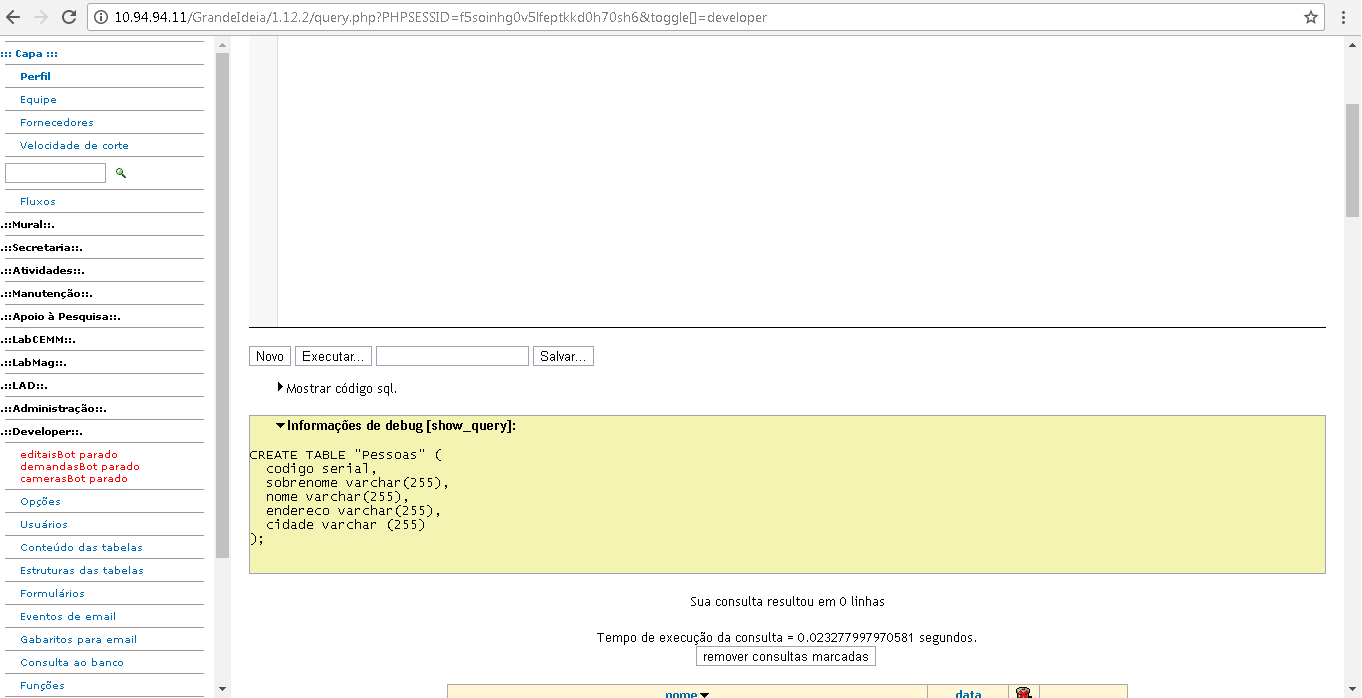
\includegraphics[width=\textwidth]{1_Consulta_ao_banco_shell_interativo/2_Criando_tabelas/6.png}.      
      \caption{Debug.}
      \label{fig:Debug}
    \end{figure}

    Caso haja algum erro, o sistema reportará e indicará a linha
    do código onde ele está localizado. A quantidade de
    informações sobre o código dependerá do nível de debug
    selecionado. Como alterar o nível de debug é explicado
    no Capítulo \textbf{Opções}.

    \subsection{Consultando o banco de dados}

    Além de criar tabelas, o shell interativo pode ser usado
    para consultar, incluir linhas, colunas e excluir tabelas
    do banco de dados. Para realizar tais ações é utilizada a
    sintaxe padrão do SQL, portanto, as mesmas regras citadas
    na criação de tabela serão válidas para demais funções no
    banco de dados. Veja exemplos de utilização dos comandos
    \texttt{\textbf{SELECT}} e \texttt{\textbf{INSERT}}.
    Primeiro, vamos inserir dados a tabela.
     \\
    
    \underline{\textbf{Passo 1:}}  Digite o comando para inserção
    respeitando a devida sintaxe:

   \begin{lstlisting}
     INSERT INTO table_name VALUES (column1, column2, column3, columnN );
   \end{lstlisting}
   
   Utilizando a tabela criada para exemplo, teremos:
   
   \begin{lstlisting}
     INSERT INTO "Pessoas" VALUES (1, 'Leal', 'Gustavo', 'Av. Ipiranga, 6681', 'Porto Alegre');
   \end{lstlisting}

   \begin{figure}[H]
      %-%\includegraphics[width=\textwidth]{1_Consulta_ao_banco_shell_interativo/3_Consultando_tabelas/7.png}.
      \caption{Inserção de dados.}
      \label{fig:inserindoDados}
   \end{figure}

   \begin{figure}[H]
      %-%\includegraphics[width=\textwidth]{1_Consulta_ao_banco_shell_interativo/3_Consultando_tabelas/8.png}.      
      \caption{Executando Inserção.}
      \label{fig:executarIn}
   \end{figure}

   \begin{figure}[H]
     %-%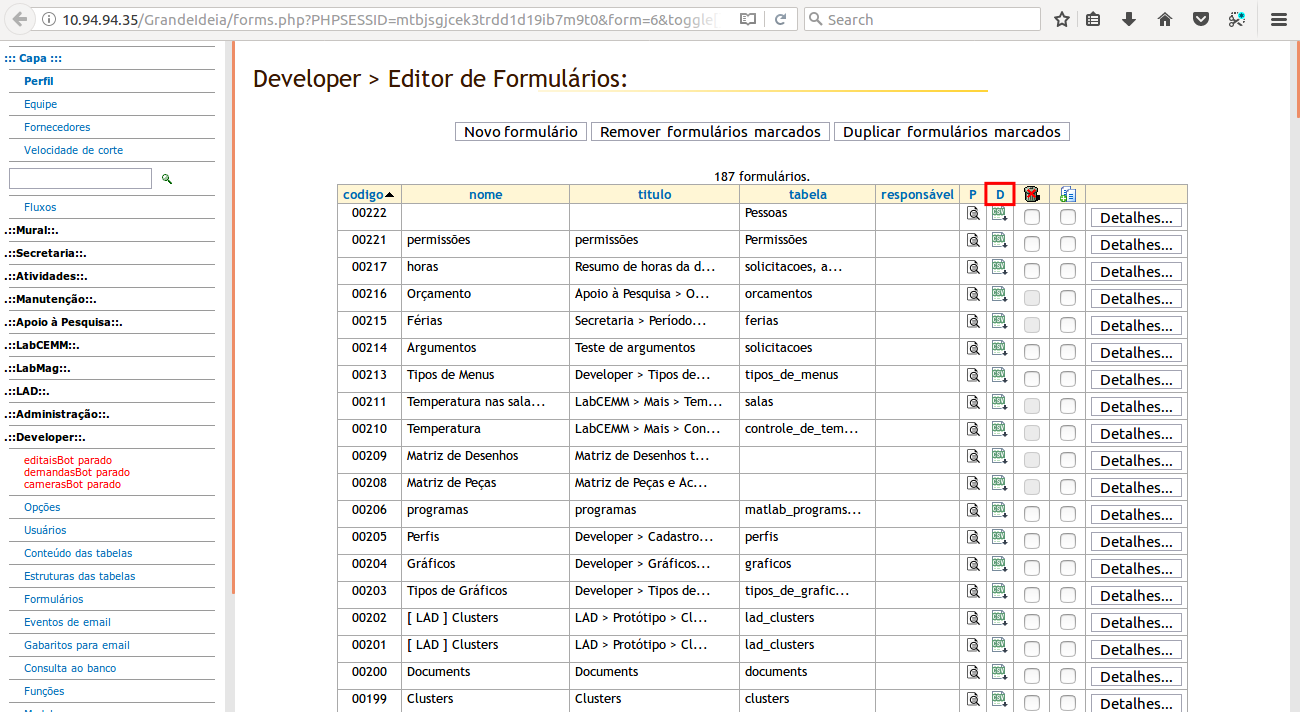
\includegraphics[width=\textwidth]{1_Consulta_ao_banco_shell_interativo/3_Consultando_tabelas/9.png}     
     \caption{Debug.}
     \label{fig:debugInsercao}
   \end{figure}

   Em informações de debug, confira se não houve erros na inserção.
   Agora é possível consultar a tabela utilizando o comando
   \texttt{\textbf{ SELECT}}, conforme exemplo.
   \\
   \begin{lstlisting}
     SELECT * FROM "Pessoas";
   \end{lstlisting}
  
  \begin{figure}[H]
     %-%\includegraphics[width=\textwidth]{1_Consulta_ao_banco_shell_interativo/3_Consultando_tabelas/10.png}     
     \caption{Consultando tabela.}
     \label{fig:select1}
   \end{figure}

   \begin{figure}[H]
     %-%\includegraphics[width=\textwidth]{1_Consulta_ao_banco_shell_interativo/3_Consultando_tabelas/11.png}    
     \caption{Executando consulta.}
     \label{fig:execons}
   \end{figure}

    \begin{figure}[H]
     %-%\includegraphics[width=\textwidth]{1_Consulta_ao_banco_shell_interativo/3_Consultando_tabelas/12.png}     
     \caption{Debug e resultado.}
     \label{fig:select2}
    \end{figure}

    Após executar o comando, verifique se não houve erros em
    \textbf{Informações de debug}. Abaixo de \textbf{Informações de
     debug}, uma tabela deverá aparecer. Esta tabela é o resultado do
    comando \texttt{\textbf{SELECT}}, sendo apresen tada a tabela
    criada anteriormente. Para visualizar apenas uma coluna ou
    determinados campos, basta substituir o comando “ * “ da linha d
    e código pela coluna desejada e/ou acrescentar
    \texttt{\textbf{WHERE}} ao final, seguido pela condição desejada.
    
    \section{Conteúdo, estrutura e modelo de tabelas}
    
    É possível visualizar o conteúdo e a estrutura das tabelas sem
    realizar uma consulta ao banco por meio do shell. O framework
    ONDE possui dois menus para isso: \textbf{Conteúdo das tabelas} e
    \textbf{Estrutura das tabelas}. Ambos ficam localizados no menu
    \textbf{Developer}, no lado esquerdo da tela.

    Acesse \textbf{Conteúdo das tabelas} no lado esquerdo da tela.

    \begin{figure}[H]
     %-%\includegraphics[width=\textwidth]{1_Consulta_ao_banco_shell_interativo/4_conteudo_e_estrutura_tabelas/13.png}     
     \caption{Conteúdo das tabelas.}
     \label{fig:conttabelas}
    \end{figure}

    Você verá a lista de tabelas existentes no banco de dados. Será
    apresentado o nome da tabela (\textbf{tablename}), o dono da
    tabela (\textbf{tableowner}), o número de linhas
    (\textbf{linhas}) e a opção Detalhes para visualizar o conteúdo.
    Clique em \textbf{Detalhes} ao lado de uma tabela.
    
    \begin{figure}[H]
     %-%\includegraphics[width=\textwidth]{1_Consulta_ao_banco_shell_interativo/4_conteudo_e_estrutura_tabelas/14.png}
     \caption{Tabela Pessoas.}
     \label{fig:conttabelapes}
    \end{figure}

    Acessamos a tabela Pessoas. Veja que ela possui uma(1) linha.
    Agora, vamos acessar o menu Estrutura das tabelas.

    \begin{figure}[H]
     %-%\includegraphics[width=\textwidth]{1_Consulta_ao_banco_shell_interativo/4_conteudo_e_estrutura_tabelas/15.png}
     \caption{Estrutura das tabelas.}
     \label{fig:estruturatabelas}
    \end{figure}

    Esta visualização possui 3 colunas: \textbf{oid}, o nome da
    tabela (\textbf{tablename}) e o número de linhas
    (\textbf{linhas}). Também possui o botão \textbf{Detalhes}.
    Clique nele ao lado de uma tabela. Vamos escolher a mesma
    anterior, a tabela \textbf{Pessoas}.

    \begin{figure}[H]
     %-%\includegraphics[width=\textwidth]{1_Consulta_ao_banco_shell_interativo/4_conteudo_e_estrutura_tabelas/16.png}
     \caption{Estrutura da tabela Pessoas.}
     \label{fig:estruturapessoas}     
    \end{figure}
    
    Agora você pode visualizar a estrutura da tabela. Isto é, o nome
    , o tipo e o limite de cada coluna. É possível verificar a
    estrutura de qualquer coluna através deste método. Vamos procurar
    a tabela  \textbf{forms}, onde estão armazenados todos os
    formulários criados pelo  \textbf{Editor de formulários}. Utilize
    a ferramenta de pesquisa do navegador com o comando
    \textbf{CTRL+F} e digite o nome da tabela desejada.

     \begin{figure}[H]
     %-%\includegraphics[width=\textwidth]{1_Consulta_ao_banco_shell_interativo/4_conteudo_e_estrutura_tabelas/17.png}
     \label{fig:festruturaforms}
     \caption{Localizando a tabela forms.}
    \end{figure}

     Note que ela possui 192 linhas, referindo-se ao número de dados
     inseridos nela, visíveis no menu \textbf{Conteúdo das tabelas}.
     Clique em \textbf{Detalhes} ao lado dela.

     \begin{figure}[H]
     %-%\includegraphics[width=\textwidth]{1_Consulta_ao_banco_shell_interativo/4_conteudo_e_estrutura_tabelas/18.png}
     \caption{Estrutura da tabela forms.}
     \label{fig:estruturaforms}
     \end{figure}
     
     Esta é a estrutura da tabela \textbf{Forms}. Você verá que o
     nome destas colunas estão presentes no \textbf{Editor de
       Formulários} para inclusão de novos formulários, que será
     contemplado no próximo capítulo.

     O \textbf{modelo} de um banco de dados demonstra a estrutura e
     os relacionamentos entre tabelas. O framework O.N.D.E possui um
     menu para visualização deste modelo em gráfico. Para acessá-lo,
     clique no menu \textbf{Modelo} no lado esquerdo da tela.

      \begin{figure}[H]
     %-%\includegraphics[width=\textwidth]{1_Consulta_ao_banco_shell_interativo/4_conteudo_e_estrutura_tabelas/19.png}
     \caption{Modelo do banco de dados.}
     \label{fig.modelo}
     \end{figure}

      É possível movimentar-se pelo Modelo clicando e arrastando com
      o mouse. Você verá a ligação entre todas as tabelas do banco
      de dados por meio das \textbf{linhas azuis}. Também é possível
      movimentar as tabelas e reorganizar o modelo como desejar,
      clicando sobre uma tabela e arrastando.

      %%%%%%%%%%%%%%%%%%%%%%%%%%%%%%%%%%%%%%%%%%%%%%%%%%%%%%%%%%%
      %%%%%%%%%%%%%%%%%%%%%%%%%%%%%%%%%%%%%%%%%%%%%%%%%%%%%%%%%%%
   \chapter{Formulários}
   
   O framework O.N.D.E sistema Grande IDEIA é padronizado por
   formulários criados pelos desenvolvedores com a finalidade de
   facilitar o processo de inclusão e alteração de relatórios. Todos
   os relatórios são criados a partir de um modelo na tabela
   \textbf{forms}, incluindo o próprio \textbf{editor de formulários}
   onde são criados os demais.
   
   Para acessar a gestão de formulários, basta seguir o caminho
   através do menu \textbf{Developer}, conforme mostram as Figuras
   \figurename{ \ref{fig:capa}} e \figurename{ \ref{fig:editorf}}.

    \begin{figure}[H]
      %-%
\includegraphics[width=\textwidth]{2_Formularios/1_Editor_de_formularios/1.png}
      \caption{Página inicial.}
      \label{fig:capa}
    \end{figure}

    \begin{figure}[H]
      %-%\includegraphics[width=\textwidth]{2_Formularios/1_Editor_de_formularios/2.png}
      \caption{Editor de Formulários.}
      \label{fig:editorf}
    \end{figure}

   \section{Editor de formulários}

   O \textbf{Editor de formulários} é uma interface criada para gerar
   os formulários que vão atuar no sistema. Todos os formulários são
   baseados em um modelo definido no arquivo forms.php, inclusive o
   próprio editor. Portanto, é possível localizá-lo na tabela de
   formulários e editar conforme necessário. Para criar novos
   formulários, basta clicar no botão \textbf{Novo formulário}.

    \begin{figure}[H]
      %-%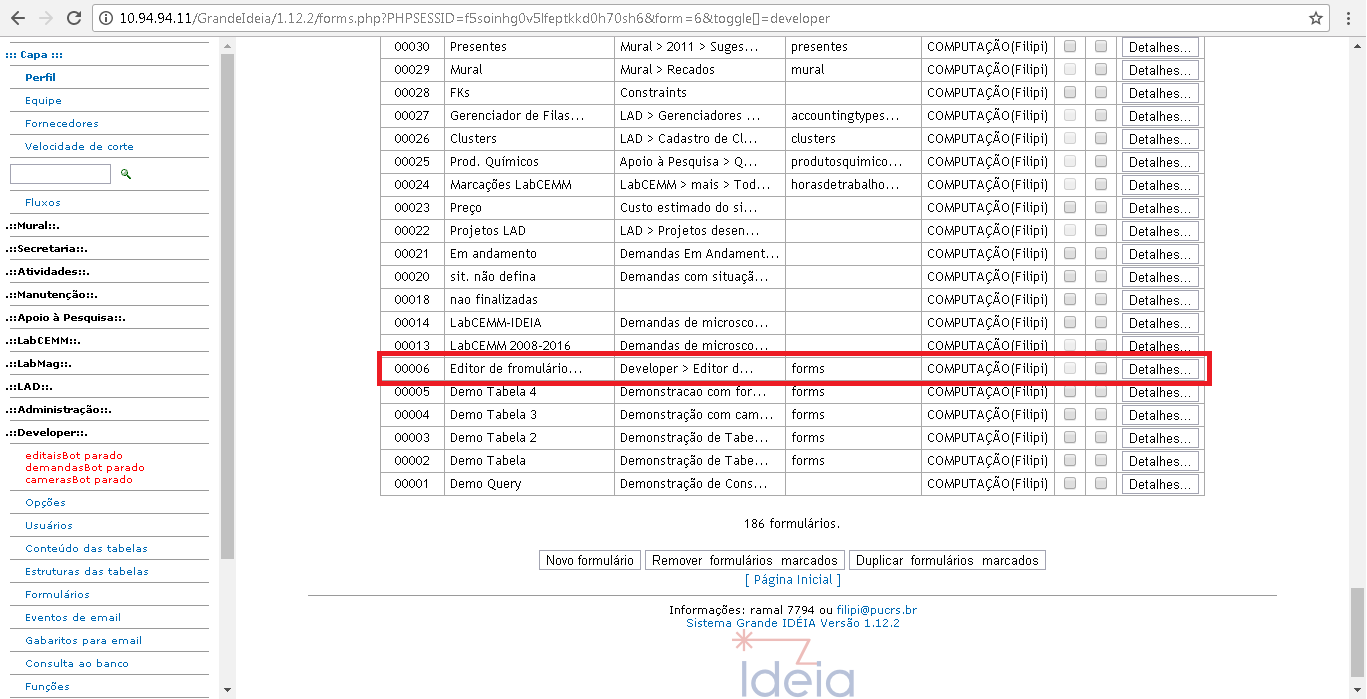
\includegraphics[width=\textwidth]{2_Formularios/1_Editor_de_formularios/3.png}
      \caption{Novo formulário.}
      \label{fig:novoform}
    \end{figure}

    Ao clicar em \textbf{Novo formulário} você será redirecionado
    para o o \textbf{Editor de formulários}. A coluna com o símbolo
    de lixeira tem a função de remover um formulário da tabela.
    Primeiro é marcada a checkbox referente ao formulário desejado,
    para depois clicar em \textbf{Remover formulários marcados}.
    É possível configurar os formulários para proteger contra
    remoção, explicado na seção sobre criação de formulários.

    \begin{figure}[H]
      %-%
\includegraphics[width=\textwidth]{2_Formularios/1_Editor_de_formularios/4.png}
      \caption{Remover formulários.}
      \label{fig:removerform}
    \end{figure}

    Além de criar e remover formulário, é possível  duplicar um
    formulário existente. Ao lado da coluna \textbf{Remover}
    encontra-se a coluna de duplicação. Marcando o checkbox ao lado
    do formulário desejado e clicando em
    \textbf{Duplicar formulários marcados}, gerando uma cópia do
    mesmo.
    
    \begin{figure}[H]
      %-%
\includegraphics[width=\textwidth]{2_Formularios/1_Editor_de_formularios/5.png}
      \caption{Duplicar formulários.}
      \label{fig:duplicarform}
    \end{figure}
    
    A coluna \textbf{P} tem a função de preview. Existem duas
    maneiras de visualizar um formulário: a primeira é clicando no
    ícone da coluna \textbf{P} ao lado do formulário desejado. A
    segunda é acessando o menu \textbf{Forms} no lado esquerdo da
    tela e selecionando o formulário conforme o nome dado na criação.
    Isto será abordado posteriormente.
    
    \begin{figure}[H]
      %-%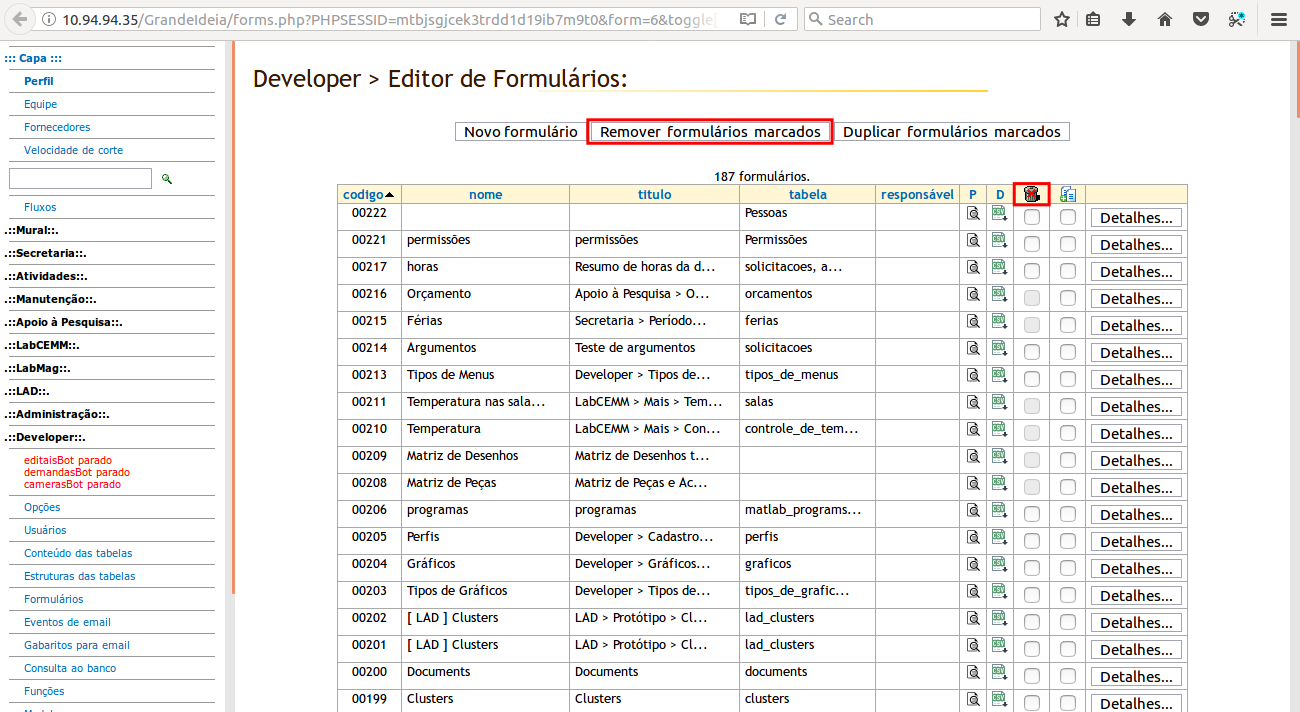
\includegraphics[width=\textwidth]{2_Formularios/1_Editor_de_formularios/6.png}
      \caption{Visualização do formulário.}
      \label{fig:preview}
    \end{figure}

    O fLamework O.N.D.E também possui da função de exportação para
    arquivo CSV com direcionamento ao \textbf{Excel}. Com isso é
    possível realizar o download da tabela para ser editada ou
    reaproveitada em outras funções dentro do Excel. A coluna
    \textbf{D} realiza o download do formulário no
    \textbf{Editor de formulários}. Desta forma, apenas o
    \textbf{desenvolvedor} poderá realizar o download. Para que todos
    os usuários deste formulário possam acessar a função é necessário
    que esta seja configurada. Como configurar esta função será
    explicado durante a criação de formulários.

     \begin{figure}[H]
      %-%\includegraphics[width=\textwidth]{2_Formularios/1_Editor_de_formularios/7.png}
      \caption{Exportar formulários para Excel.}
      \label{fig:exportExcel}
     \end{figure}

     Para editar formulários já criados, basta localizar o formulário
     desejado e clicar em \textbf{Detalhes} ao lado direito da tabela.

     \begin{figure}[H]
      %-%\includegraphics[width=\textwidth]{2_Formularios/1_Editor_de_formularios/8.png}
      \caption{Editando formulários.}
      \label{fig:detalhesForms}
     \end{figure}
        
     \section{Criação de formulários}

     Como explicado anteriormente, para criar um novo formulário é
     preciso acessar o \textbf{Editor de Formulários} e então clicar
     em \textbf{Novo Formulário}. Após isso, você será redirecionado
     para a tela de criação de formulários. O framework O.N.D.E
     possibilita a inserção de diversas funcionalidades, tais como
     envios de e-mails, edições de layout e estilização, etc. Cada
     campo de criação e edição do formulário será explicado e
     exemplificado. Primeiro iremos criar um formulário simples
     utilizando a tabela \textbf{Pessoas} criada no
     \textbf{Capítulo 7}, onde será possível registrar, excluir e
     exportar para CSV. Também serão abordados os formulários para
     tabelas com relacionamentos entre si, consultas específicas,
     envios de email e inclusão de JavaScript e HTML.

      \subsection{Formulário simples}

      No \textbf{Editor de Formulários} clique em
      \textbf{Novo Formulário} para ser redirecionado para a página
      de criação e edição.

     \begin{figure}[H]
      %-%\includegraphics[width=\textwidth]{2_Formularios/2_Criacao_de_formularios/3.png}
      \caption{Criando formulários.}
      \label{fig:editorform}
     \end{figure}

     \underline{\textbf{Passo 1:}} Preencha o \textbf{Nome} e o
     \textbf{Título} conforme o formulário. Neste caso, estamos
     usando a tabela \textbf{Pessoas}, então vamos nomear o
     formulário conforme.
     
      \begin{figure}[H]
       %-%
\includegraphics[width=\textwidth]{2_Formularios/2_Criacao_de_formularios/4.png}
       \caption{Preenchendo Nome e Título.}
       \label{fig:nometitulo}
      \end{figure}
      
      \underline{\textbf{Passo 2:}} Localize os campos
      \textbf{Tabela} e \textbf{Campos}, conforme a Figura
      \ref{campotabela}.
      
      \begin{figure}[H]
       %-%
\includegraphics[width=\textwidth]{2_Formularios/2_Criacao_de_formularios/5.png}
       \caption{Tabela e Campos.}
       \label{fig:campotabela}
      \end{figure}
      
      Preencha-os o primeiro campo com a tabela a qual o formulário
      irá realizar consultas. O segundo deve ser preenchido com as
      colunas da tabela. Não é necessário utilizar aspas duplas para
      diferenciar nomes com letras maiúsculas ou caracteres especiais
      .
      Como explicado na criação da tabelas via shell interativo, o
      fLamework O.N.D.E é capaz de diferenciar estes caracteres e
      realizar as consultas a partir deles. Apenas onde houver um
      shell interativo, que realizará consultas diretas, é necessário
      o uso de aspas. Nos \textbf{Campos}, separe o nome da colunas
      por vírgulas.

      \begin{figure}[H]
        %-%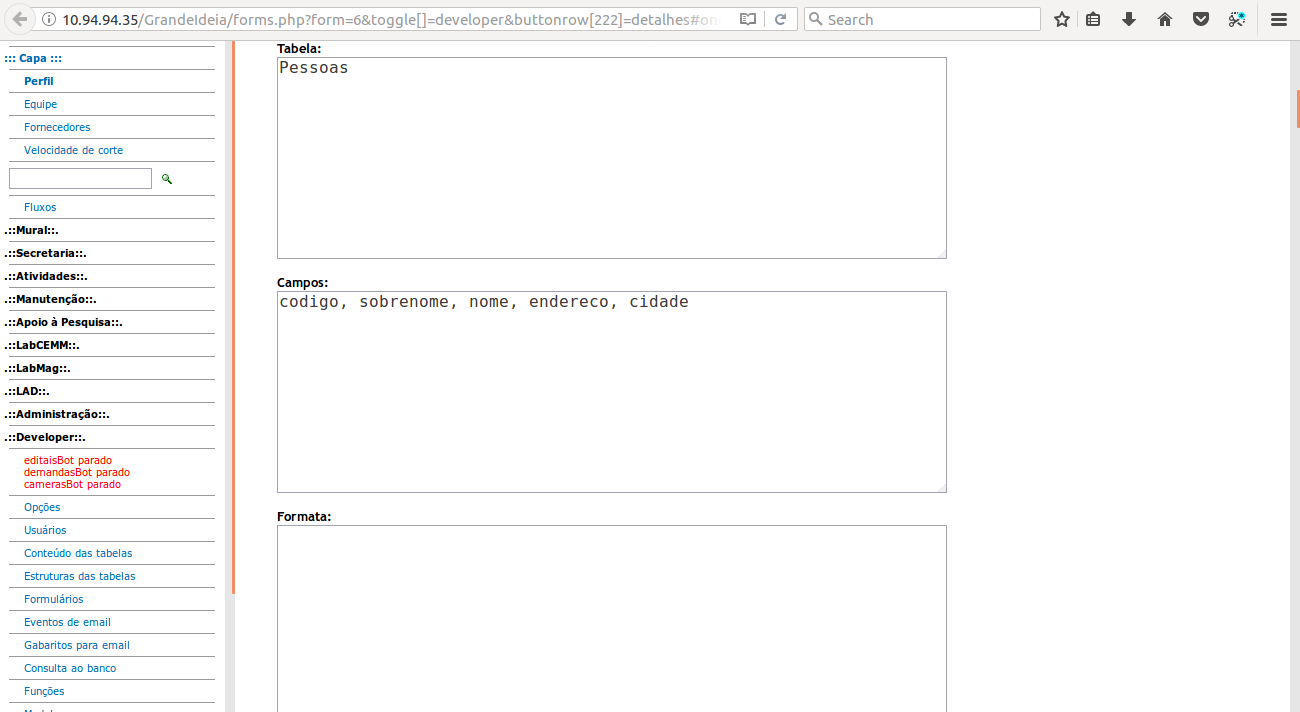
\includegraphics[width=\textwidth]{2_Formularios/2_Criacao_de_formularios/6.png}
        \caption{Exemplo de preenchimento para Tabela e Campos.}
        \label{fig:campotabela2}
      \end{figure}

      \underline{\textbf{Passo 3:}} Procure os campos
      \textbf{Funcao}, \textbf{Argumento} e \textbf{Formulario}.

      \begin{figure}[H]
        %-%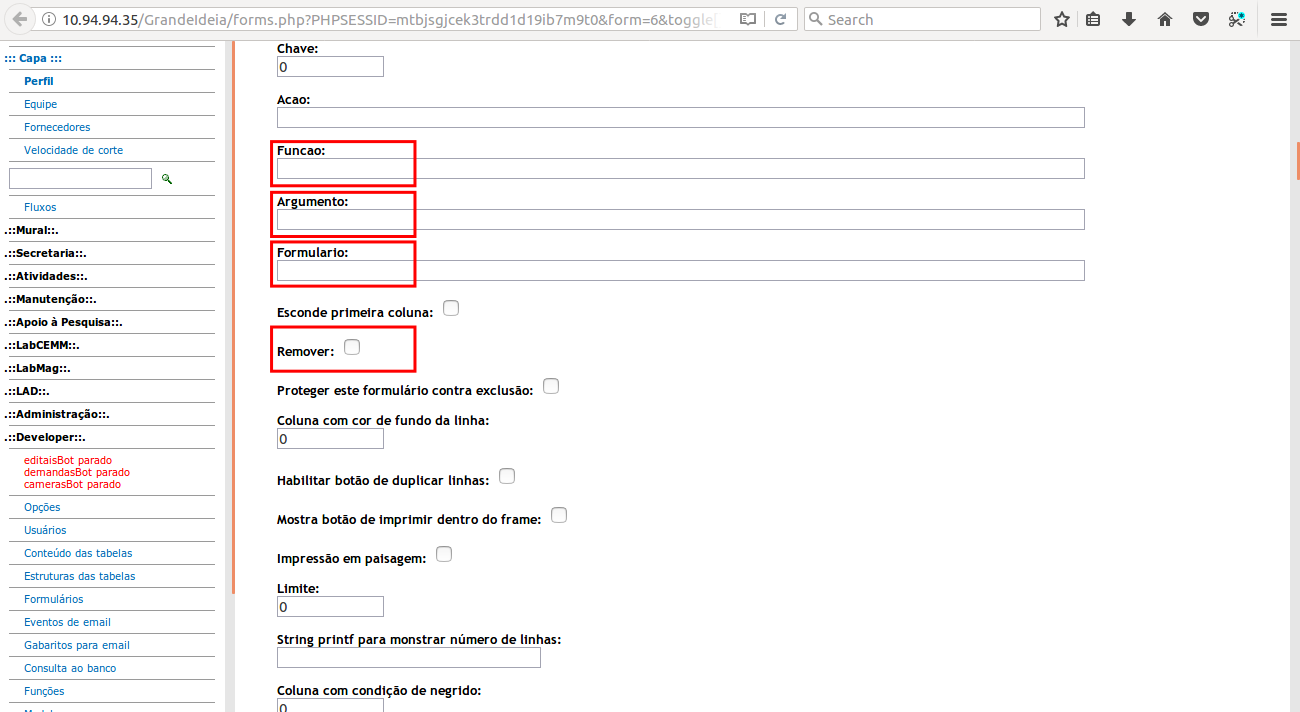
\includegraphics[width=\textwidth]{2_Formularios/2_Criacao_de_formularios/7.png}
        \label{fig:configform}
        \caption{Habilitando edições ao formulário.}
      \end{figure}

      Estes campos configuram a inclusão e a edição de dados no
      formulário. Precisam ser preenchidos em todos os formulários.
      Para casos em que haverá apenas a consulta à determinada tabela
      não são necessários. Devem ser preenchidos com os seguintes
      argumentos:
  
      \underline{\textbf{Funcao}}: basename

      \underline{\textbf{Argumento}}: \$\underline{ }SERVER[PHP\underline{ }SELF]
      
      \underline{\textbf{detalhes}}: detalhes

      \begin{figure}[H]
        %-%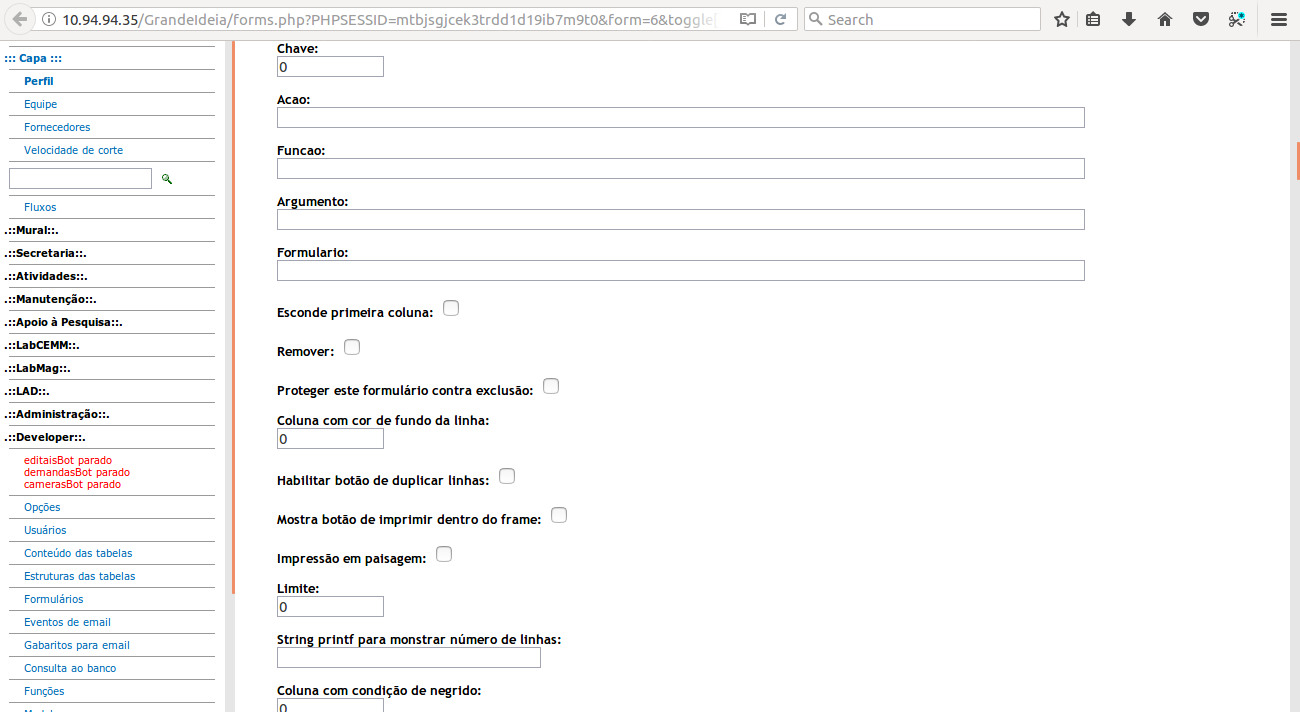
\includegraphics[width=\textwidth]{2_Formularios/2_Criacao_de_formularios/8.png}
        \caption{Funcao, Argumento e detalhes preenchidos.}
        \label{fig:configform2}
      \end{figure}

      \underline{\textbf{Passo 4:}} Vá ao final da página e
      localize o botão \textbf{Inserir}.

      \begin{figure}[H]
        %-%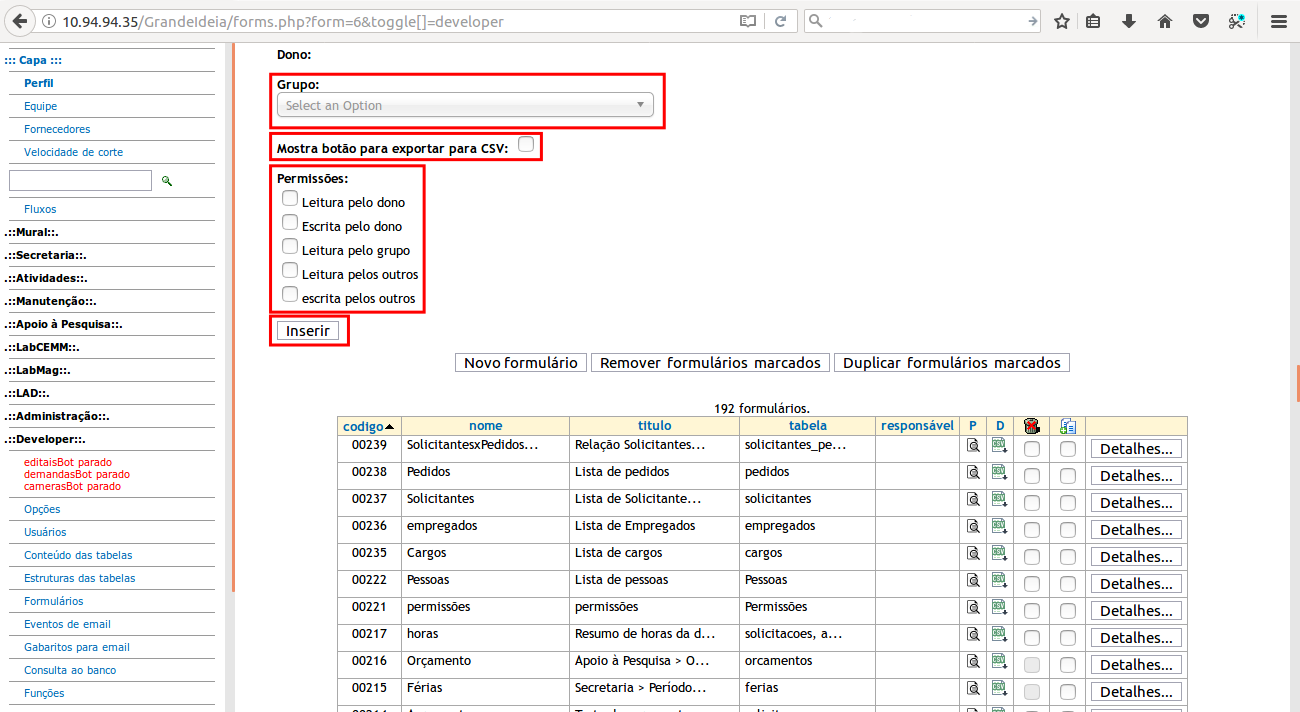
\includegraphics[width=\textwidth]{2_Formularios/2_Criacao_de_formularios/9.png}
        \caption{Final do formulário.}
        \label{fig:finalform}
      \end{figure}

      Logo antes do botão \textbf{Inserir}, localizam-se algumas
      configurações. No topo da imagem, na linha \textbf{Dono:}, é
      informado o responsável pela criação do formulário em questão.
      Será preenchido ao inserir. Abaixo, seleciona-se o grupo de
      usuários ao qual pertencerá.

      O checkbox a seguir configura o botão de exportação para CSV,
      ou seja, para Excel. Adicionará um botão na página do
      formulário, como veremos após inserirmos. Por último, as
      permissões de manipulação do formulário, que definem quem  pode
      ler ou escrever nele.

      Preencha como na \figurename{ \ref{fig:finalform2}} e clique em
      \textbf{Inserir}.

      \begin{figure}[H]
        %-%\includegraphics[width=\textwidth]{2_Formularios/2_Criacao_de_formularios/10.png}
        \caption{Pronto para inserir.}
        \label{fig:finalform2}
      \end{figure}

      Você será redirecionado para a lista de formulários e receberá
      a mensagem de sucesso no procedimento.
      
      \begin{figure}[H]
        %-%\includegraphics[width=\textwidth]{2_Formularios/2_Criacao_de_formularios/11.png}
        \caption{Formulário inserido com sucesso.}
        \label{fig:forminserido}
      \end{figure}

      \subsection{Manipulando dados pelo formulário}

      Com o formulário inserido e
      configurado é possível visualizar o mesmo como tal. Existem
      duas formas de acessar o formulário. A primeira é clicando na
      \textbf{lupa} na linha do formulário desejado, na coluna
      \textbf{P}.

      \begin{figure}[H]
        %-%\includegraphics[width=\textwidth]{2_Formularios/2_Criacao_de_formularios/12.png}
        \caption{Acessando visualização do formulário.}
        \label{fig:preview}
      \end{figure}

      Você será redirecionado para a visualização do conteúdo do
      formulário.
           
      \begin{figure}[H]
        %-%\includegraphics[width=\textwidth]{2_Formularios/2_Criacao_de_formularios/13.png}
        \caption{Visualização do formulário.}
        \label{fig:visualizacao}
      \end{figure}

      A segunda maneira de acessar o formulário é através do submenu
      \textbf{Forms} no lado esquerdo da tela, no menu
      \textbf{Developer}.

      \begin{figure}[H]
        %-%\includegraphics[width=\textwidth]{2_Formularios/2_Criacao_de_formularios/14.png}
        \caption{Acessando através do menu Forms.}
        \label{fig:Forms}
      \end{figure}

      \underline{\textbf{Passo 1:}} Para inserir novos dados ao
      formulário, clique em \textbf{Novo}.

      \begin{figure}[H]
        %-%\includegraphics[width=\textwidth]{2_Formularios/2_Criacao_de_formularios/15.png}
        \caption{Inserindo novos dados via formulário.}
        \label{fig:novosdados}
      \end{figure}
      
      Você será redirecionado a paǵina do formulário em si, onde
      poderão ser preenchidos os dados de acordo com as colunas da
      tabela.
      
      \begin{figure}[H]
        %-%\includegraphics[width=\textwidth]{2_Formularios/2_Criacao_de_formularios/16.png}
        \caption{Formulário de inserção de dados.}
        \label{fig:inserdados}
      \end{figure}

      Preencha os dados conforme necessário, como no exemplo da \figurename{ \ref{fig:prdados}}.
      
      \begin{figure}[H]
        %-%\includegraphics[width=\textwidth]{2_Formularios/2_Criacao_de_formularios/17.png}
        \caption{Preenchendo dados do formulário.}
        \label{fig:prdados}
      \end{figure}

      Terminando de inserir os dados, basta clicar em
      \textbf{Inserir} abaixo dos campos de texto. A página será
      redirecionada para a visualização do conteúdo com uma mensagem
      de sucesso e uma nova linha adicionada contendo os dados
      inseridos.

      \begin{figure}[H]
        %-%\includegraphics[width=\textwidth]{2_Formularios/2_Criacao_de_formularios/18.png}
        \caption{Dados inseridos com sucesso.}
        \label{fig:insersucesso}
      \end{figure}

      \underline{\textbf{Passo 2:}} Adicionados os novos dados, é
      possível também excluí-los. Assim como na lista de formulários, para excluir uma linha de uma tabela pelo formulário, deve-se selecionar a(s) linha(s) desejada(s) e então clicar em \textbf{Remover linhas marcadas}, como mostra a \figurename{ \ref{fig:linhasexclusao}}.

      \begin{figure}[H]
        %-%\includegraphics[width=\textwidth]{2_Formularios/2_Criacao_de_formularios/19.png}
        \caption{Excluindo linha.}
        \label{fig:linhasexclusao}
      \end{figure}

      Marque a linha inserida anteriormente e clique em \textbf{Remover linhas marcadas} para excluí-la.

      \begin{figure}[H]
        %-%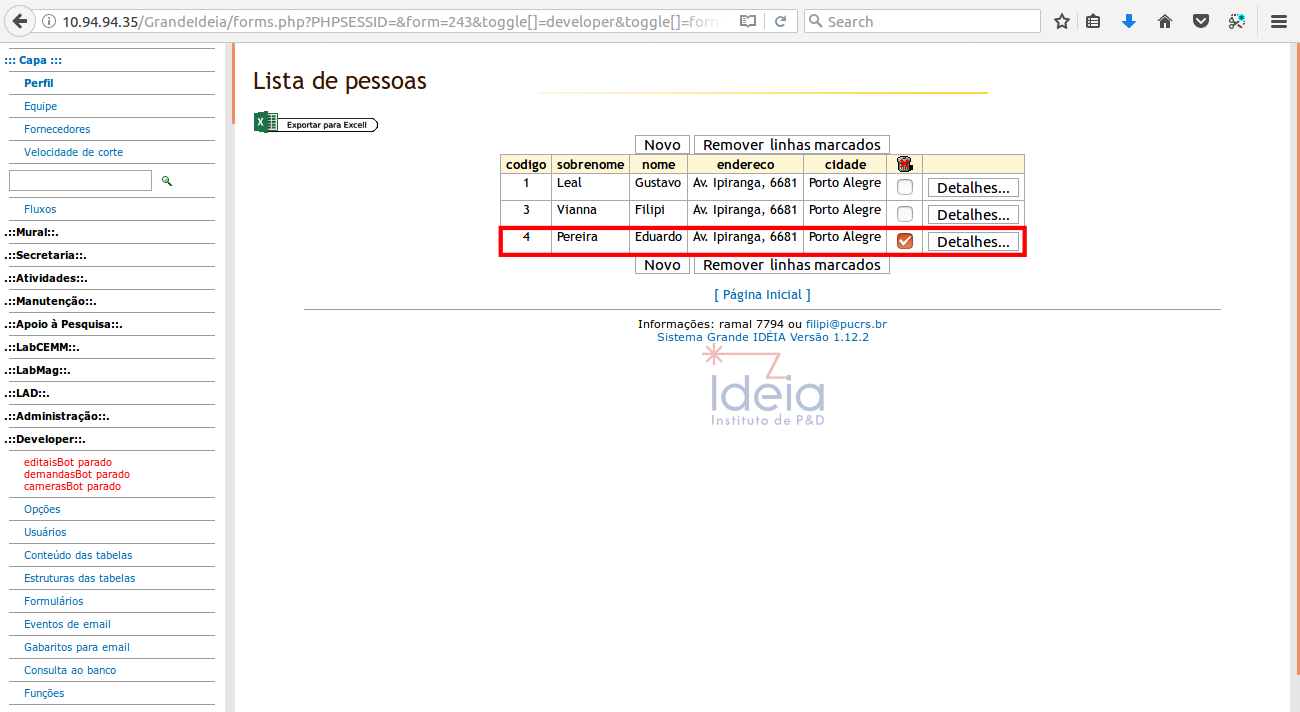
\includegraphics[width=\textwidth]{2_Formularios/2_Criacao_de_formularios/20.png}
        \caption{Marcando linhas para exclusão.}
        \label{fig:linhamarcada}
      \end{figure}
      
      Uma mensagem de sucesso na exclusão deverá aparecer na tela de
      visualização dos dados e a linha deverá desaparecer.
      
      \begin{figure}[H]
        %-%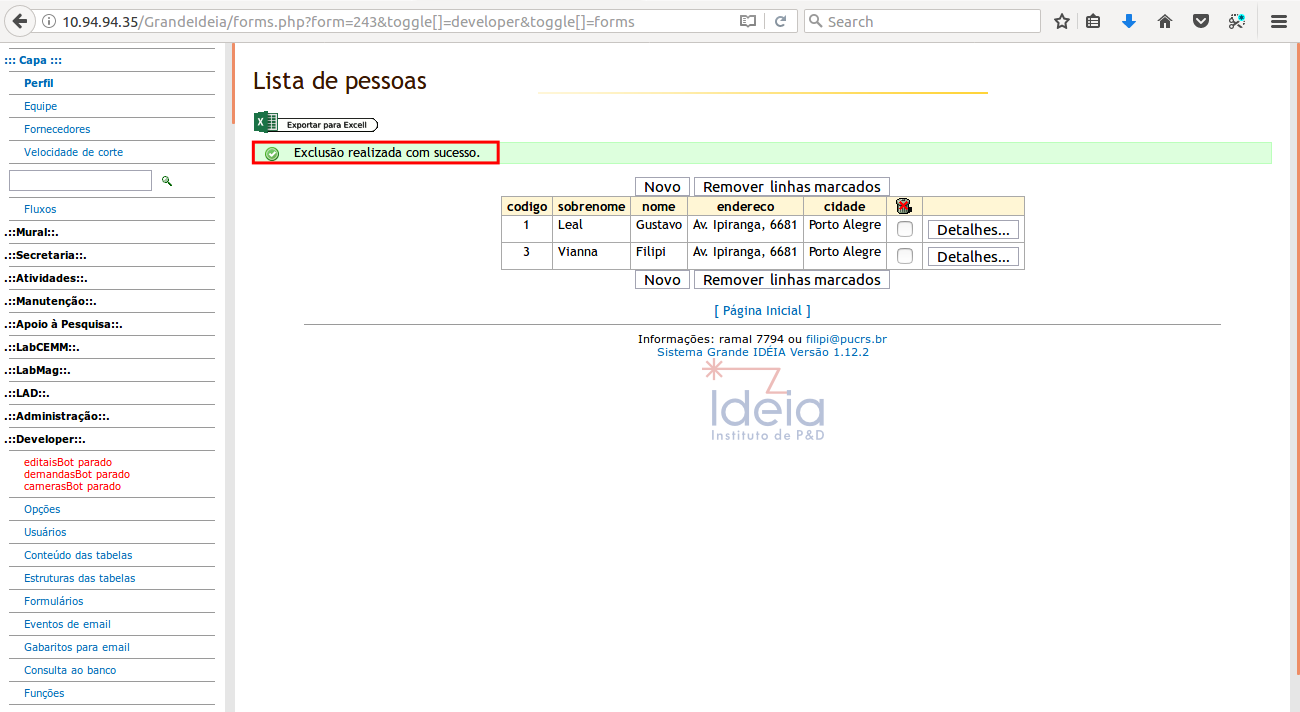
\includegraphics[width=\textwidth]{2_Formularios/2_Criacao_de_formularios/21.png}
        \caption{Exclusão realizada com sucesso.}
        \label{fig:exclusaosucesso}
      \end{figure}

      \underline{\textbf{Passo 3:}} Abaixo do título dado ao
      formulário encontra-se o botão de exportação para Excel, no
      formato CSV. Lembrando que o botão está ativo devido ao
      checkbox marcado na criação do formulário, logo antes das
      permissões de usuários.

      \begin{figure}[H]
        %-%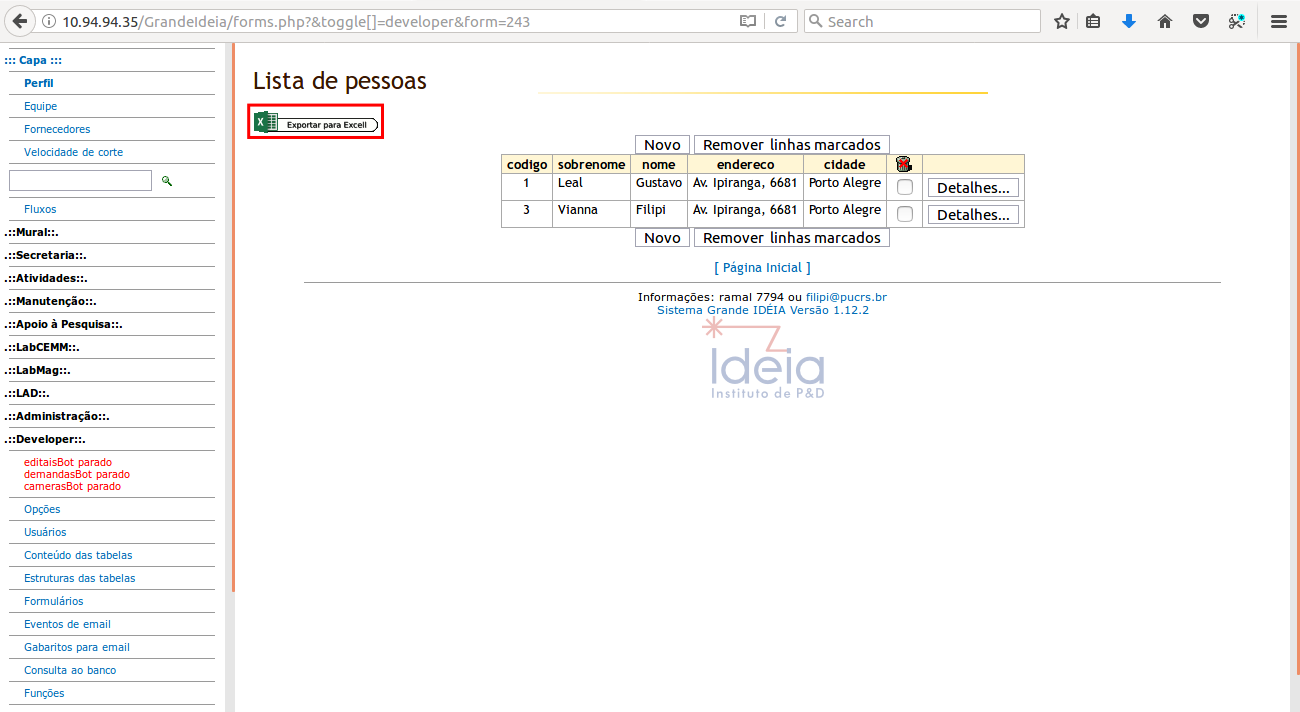
\includegraphics[width=\textwidth]{2_Formularios/2_Criacao_de_formularios/22.png}
        \caption{Exportação para Excel.}
        \label{fig:exportexcel}
      \end{figure}

      Ao clicar no botão o download do arquivo será inicializado. Conforme as opções do seu navegador, poderá iniciar direto ou perguntar se deve salvar ou abrir o arquivo.

      \begin{figure}[H]
        %-%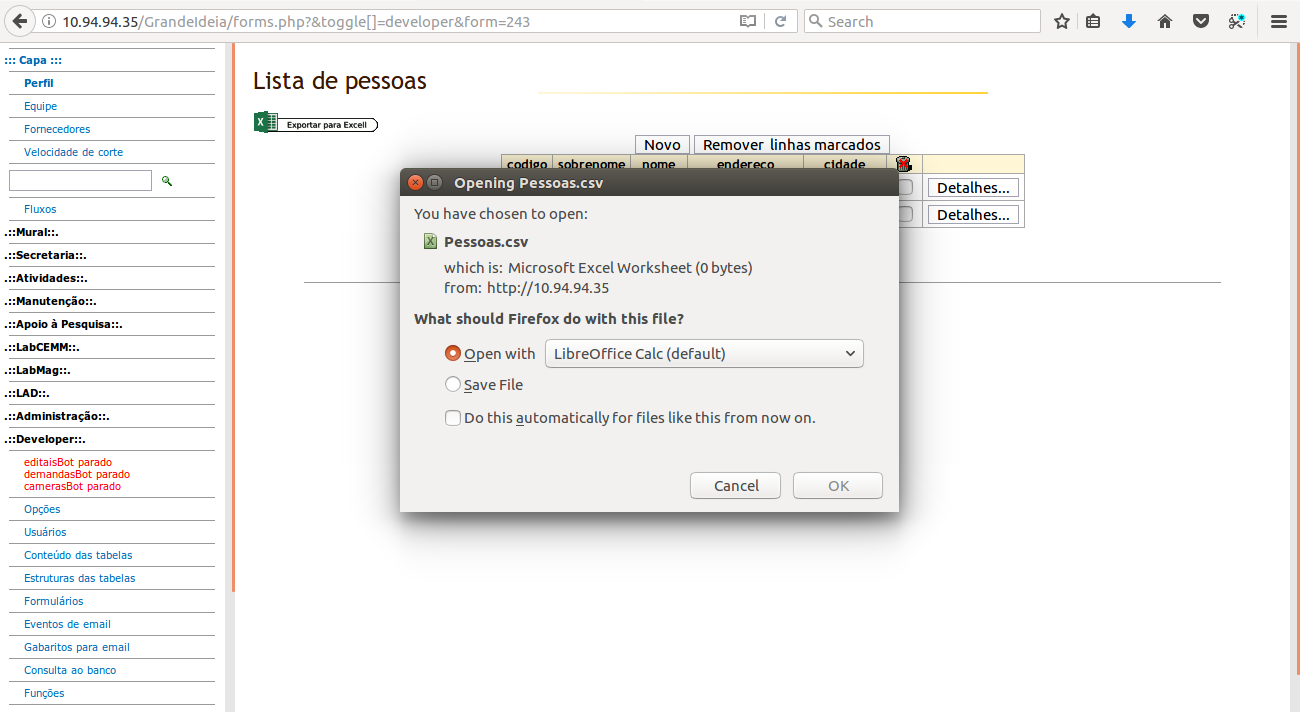
\includegraphics[width=\textwidth]{2_Formularios/2_Criacao_de_formularios/23.png}
        \caption{Download do arquivo .csv.}
        \label{fig:downloadcsv}
      \end{figure}

      Ao abrir o arquivo, algumas configurações serão necessárias na
      janela de opções que abrirá, conforme \figurename{ {\ref:abrindocsv}}. 

      \begin{figure}[H]
        %-%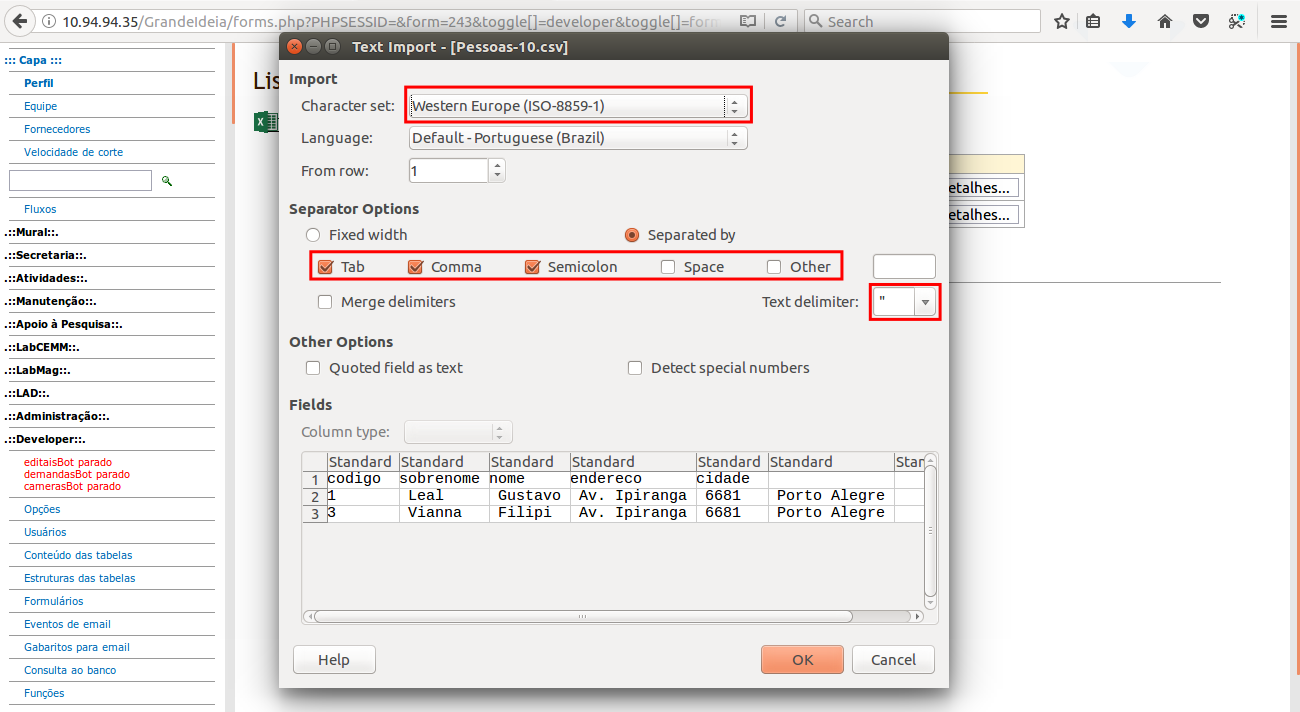
\includegraphics[width=\textwidth]{2_Formularios/2_Criacao_de_formularios/24.png}
        \caption{Configurando a leitura do arquivo CSV.}
        \label{fig:abrindocsv}
      \end{figure}

      Faça as seguintes modificações nesta janela:
      \\
      
      \underline{\textbf{Character set}}: altere para Western Europe
      (ISO-8859-1);

      \underline{\textbf{Separator Option}}: Desmarque todas as
      caixas;
      
      \underline{\textbf{Text delimiter}}: Deixe preenchido com uma
      aspa dupla (").
      \\

      Também é exibida uma pré-visualização da tabela. Após feitas as
      modificações, clique em \textbf{ok}.

      \begin{figure}[H]
        %-%\includegraphics[width=\textwidth]{2_Formularios/2_Criacao_de_formularios/25.png}
        \caption{Formulário exportado para excel.}
        \label{fig:exportexcelfim}
      \end{figure}
   
      \subsection{Formulário com relacionamentos}
      
      Formulários com relacionamentos utilizam informações de outras tabelas
      associadas às colunas da sua tabela principal. Para criar um formulário
      com relacionamento primeiro criamos as tabelas a serem relacionadas,
      incluindo o relacionamento, via SQL. O Framework O.N.D.E possui algumas
      particularidades para que os relacionamentos sejam apresentados nos
      formulários. Portanto, criaremos dois tipos de relacionamentos
      (\textbf{1:N, N:N}).
      
      \subsubsection{Formulários com relacionamento 1:N}
      
      Para exemplificar o relacionamento 1:N criaremos duas tabelas
      chamadas empregados e cargos. A criação seguirá o padrão
      demonstrado no \textbf{seção 7.1 Shell interativo}.

      \underline{\textbf{Passo 1:}}Acesse o menu Consulta ao banco e
      entre com o seguinte código para criar a tabela Cargos:

      \begin{lstlisting}
        CREATE TABLE cargos (
           codigo serial,
           descricao VARCHAR(255),
           salario FLOAT(24)
        );
      \end{lstlisting}

      \begin{figure}[H]
        %-%\includegraphics[width=\textwidth]{2_Formularios/3_Relacionamento_1_N/26.png}
        \caption{Criando tabela Cargos.}
        \label{fig:criatablecargos}
      \end{figure}

      Clique em \textbf{Executar} para finalizar e verifique as \textbf{Informações de debug}. A primeira tabela está criada.

      \underline{\textbf{Passo 2:}} Para criar a tabela empregados
      entre com o código:

      \begin{lstlisting}
        CREATE TABLE empregados (
           codigo serial,
           nome VARCHAR(255),
           endereco VARCHAR(255),
           cargo INTEGER REFERENCES cargos(codigo)
        );
      \end{lstlisting}

      A coluna cargo está selecionada para o tipo
      \texttt{\textbf{INTEGER}}, pois os tipos de dados entre a
      coluna referenciada e a coluna referência devem ser
      compatíveis. Utilizamos o comando \texttt{\textbf{REFERENCES}},
      pertencente ao banco de dados \textbf{PostgreeSQL}, utilizado
      neste manual, para criar uma relação com a tabela
      \textbf{cargos} e a coluna \textbf{codigo}. Sendo assim, o
      conteúdo da coluna \textbf{cargo}, da tabela
      \textbf{empregados}  será preenchido pelo conteúdo da tabela
      \textbf{cargos} de acordo com o codigo referente. Sendo assim,
      se entrarmos com o codigo 1 na coluna cargo da tabela
      empregados, o cargo deste empregado será a linha relacionada
      ao codigo 1 da tabela cargos. Sendo assim, um \textbf{cargo}
      poderá pertencer a diversos \textbf{empregados}, mas cada
      empregado terá apenas um cargo.

      \begin{figure}[H]
        %-%\includegraphics[width=\textwidth]{2_Formularios/3_Relacionamento_1_N/27.png}
        \caption{Criando tabela empregados.}
        \label{fig:criatableempregados}
      \end{figure}
      
      \underline{\textbf{Passo 3:}} Criadas as tabelas com o devido
      relacionamento, geramos os formulários utilizando o
      \textbf{editor de formulários}. Acesse o menu Formulários,
      clique em \textbf{Novo formulário} e crie um formulário simples
      referente a cada tabela seguindo o mesmo padrão utilizado em
      \textbf{8.2.1 - Criação de formulários}.
      
      \begin{figure}[H]
        %-%\includegraphics[width=\textwidth]{2_Formularios/3_Relacionamento_1_N/28.png}
        \caption{Formulários Lista de Empregados e Lista de Cargos.}
        \label{fig:listaempregadoscargos}
      \end{figure}

      \underline{\textbf{Passo 4:}} Para os relacionamentos
      funcionarem adequadamente, é necessário configurar as captions
      (legendas) dentro do \textbf{Editor de Formulários}. Em um
      relaciomento 1:N, como o desta etapa do manual, é preciso
      acessar o editor no formulário da tabela com relação 1. Neste
      caso, o formulário \textbf{Lista de Empregados}, no qual cada
      empregado cadastrado terá apenas um cargo, que será selecionado
      em uma lista que recebe os dados da tabela \textbf{cargos}.

      Para realizar essa configuração, clique em \textbf{Detalhes} ao
      lado do formulário \textbf{Lista de Empregados}. No
      \textbf{Editor de Formulários}, procure o campo
      \textbf{Reference Captions}. Para preencher esse campo, devemos
      ter em mente duas informações: qual coluna receberá as
      informações de outra tabela e qual coluna desta outra tabela
      usaremos para identificar os dados na que receberá. Neste caso,
      a coluna \textbf{cargo} da tabela \textbf{empregado} receberá
      as informações da tabela \textbf{cargos}. E para identificar as
      informações da tabela cargos, o ideal é usarmos a
      \textbf{descricao} do cargo. Agora, analise a posição da coluna
      \textbf{cargo} na tabela \textbf{empregado}. Ela é a quarta
      coluna da tabela. Sendo assim, iremos identificar ela
      adicionando uma vírgula para cada coluna anterior a tabela
      desejada. Ao chegar na posição, inserimos o nome da coluna que
      representará os dados de outra tabela, neste caso, a coluna
      \textbf{descricao} da tabela \textbf{cargos}. Veja a
      \figurename{ \ref{fig:referencecaptions}} para melhor
      entendimento.

      \begin{figure}[H]
        %-%\includegraphics[width=\textwidth]{2_Formularios/3_Relacionamento_1_N/29.png}
        \caption{Configurando reference captions.}
        \label{fig:referencecaptions}
      \end{figure}
      
      \underline{\textbf{Passo 5:}} Com os formulários criados,
      podemos adicionar informações a elas. Lembrando que há duas
      formas para acessar um formulário em si: através da coluna
      \textbf{P} na lista de formulários e através do menu
      \textbf{Forms} no lado esquerdo da tela. Primeiro vamos incluir
      alguns cargos. Acesse o formulário \textbf{Lista de cargos}.

       \begin{figure}[H]
        %-%\includegraphics[width=\textwidth]{2_Formularios/3_Relacionamento_1_N/30.png}
        \caption{Formulário Lista de cargos}
        \label{fig:listacargos}
       \end{figure}

       Clique em \textbf{Novo} para incluir um novo cargo.
       
       \begin{figure}[H]
        %-%\includegraphics[width=\textwidth]{2_Formularios/3_Relacionamento_1_N/31.png}
        \caption{Formulário para novos cargos}
        \label{fig:novoscargos}
       \end{figure}

       Preencha os campos conforme a descrição.

       \begin{figure}[H]
        %-%\includegraphics[width=\textwidth]{2_Formularios/3_Relacionamento_1_N/32.png}
        \caption{Inserindo novo cargo}
        \label{fig:novocargo}
       \end{figure}

       Após preencher, clique em Inserir e verifique se houve sucesso
       na inserção. Note que o novo cargo aparecerá ao final da lisa
       e com o código de maior valor.

       \begin{figure}[H]
        %-%\includegraphics[width=\textwidth]{2_Formularios/3_Relacionamento_1_N/33.png}
        \caption{Formulário atualizado com sucesso.}
        \label{fig:cargoinserido}
       \end{figure}

       Repita o processo e insira mais alguns cargo na tabela antes
       de prosseguir.
      
       \underline{\textbf{Passo 6:}} Acesse o formulário
       \textbf{Lista de empregados} e clique em \textbf{Novo} para
       inserir novos empregados.

       \begin{figure}[H]
        %-%\includegraphics[width=\textwidth]{2_Formularios/3_Relacionamento_1_N/34.png}
        \caption{Formulário Lista de empregados.}
        \label{fig:listaempregados}
       \end{figure}

       Veja que no campo para a coluna \textbf{cargo} temos uma caixa
       de seleção. Preencha os demais campos normalmente e clique na
       caixa de seleção.

       \begin{figure}[H]
        %-%\includegraphics[width=\textwidth]{2_Formularios/3_Relacionamento_1_N/35.png}
        \caption{Formulário para novos empregados.}
        \label{fig:novosempregados}
       \end{figure}

       \begin{figure}[H]
        %-%\includegraphics[width=\textwidth]{2_Formularios/3_Relacionamento_1_N/36.png}
        \caption{Inserindo novo empregado.}
        \label{fig:novoempregado}
       \end{figure}

       Note que as opções desta caixa de seleção são, na verdade, os
       cargos inseridos no formulário \textbf{Lista de cargos}.
       Selecione um e clique em \textbf{Inserir}.

       \begin{figure}[H]
        %-%\includegraphics[width=\textwidth]{2_Formularios/3_Relacionamento_1_N/37.png}
        \caption{Empregado inserido com sucesso.}
        \label{fig:empregadoinserido}
       \end{figure}

       Insira diversos empregados com diferentes cargos. Veja que p
       oderá repetir os cargos em diferentes empregados. Na coluna
       \textbf{cargo} estará incluso apenas o código de cada cargo,
       que se repetirá em diversas linhas. Para que seja vista a
       descrição de cada cargo é preciso que seja feita uma consulta
       específica no formulário. Como realizar consultas específicas
       estará explicado na seção
       \textbf{8.2.4 - Fomulários com consulta específica}.

       \subsubsection{Formulários com relacionamento N:N}


       %% Porque usar o \underline{ } ao invés de _ ?
       %% ass. Filipi
       O modelo relacional N:N exige a criação de 3 tabelas.
       Portanto, criaremos as tabelas \textbf{solicitantes},
       \textbf{pedidos} e \textbf{solicitantes\underline{ }pedidos}.
       Nesta relação, um cliente pode ter diversos pedidos e um
      pedido pode pertencer a diversos clientes. 

       \underline{\textbf{Passo 1:}} Acesse o shell interativo no
       menu \textbf{Consulta ao banco} e crie as tabelas utilizando
       o código abaixo.
       
       \begin{lstlisting}

         CREATE TABLE solicitantes(
           codigo serial primary key, -- uniq, NOT NULL,
           nome varchar(60) NOT NULL,
           sexo char(1) NOT NULL,
           status char(1) NOT NULL,  
           CONSTRAINT CH\underline{ }Cliente CHECK (sexo IN('F', 'M')
           )
         );
           CREATE TABLE pedidos(
           codigo serial primary key,
           produto integer,
           quantidade integer,
           data timestamp default current_timestamp
         );
         CREATE TABLE solicitantes\underline{ }pedidos(
           solicitante integer references solicitantes(codigo) on
           delete cascade,
           pedido integer references pedidos(codigo) on delete
           cascade
         );
       \end{lstlisting}
        
       \begin{figure}[H]
        %-%\includegraphics[width=\textwidth]{2_Formularios/4_Relacionamento_N_N/38.png}
        \caption{Criando tabelas para relacionamento N - N.}
        \label{fig:tabelasNN}
       \end{figure}

       \underline{\textbf{Passo 2:}} Crie um formulário para a tabela
       \textbf{solicitantes} e um para a tabela \textbf{pedidos}
       seguindo o padrão já demonstrado. Porém, para criar o
       \textbf{relacionamento N:N} é necessário preencher um campo
       extra em cada formulário. Procure por
       \textbf{Campo(s) para utilizar como etiqueta em relacoes N:N}.
       Por padrão, deve ser preenchido com a coluna \textbf{nome} da
       outra tabela que participará da relação. Nos exemplos criados,
       apenas a tabela \textbf{solicitantes} possui a coluna
       \textbf{nome}. Logo, no campo citado do formulário referente à
       tabela \textbf{pedidos}, preencheremos com a coluna
       \textbf{nome}.
       
       \begin{figure}[H]
        %-%\includegraphics[width=\textwidth]{2_Formularios/4_Relacionamento_N_N/39.png}
        \caption{Preenchendo formulário Pedidos.}
        \label{fig:formpedidosNN}
       \end{figure}

       Quando uma tabela não possui uma coluna chamada \textbf{nome},
       preenchemos com outra opção. No exemplo, a tabela
       \textbf{pedidos} não possui a coluna nome, então devemos
       preencher o campo
       \textbf{Campo(s) para utilizar como etiqueta em relacoes N:N}
       do formulário da tabela \textbf{solicitantes} com alguma outra
       coluna da tabela \textbf{pedidos}. Para exemplo, vamo usar a
       coluna código, que poderá identificar o pedido sem se repetir.

       \begin{figure}[H]
        %-%\includegraphics[width=\textwidth]{2_Formularios/4_Relacionamento_N_N/40.png}
        \caption{Preenchendo formulário Solicitantes.}
        \label{fig:formsolicitNN}
       \end{figure}

       Salve os dois formulários e prossiga.

       \underline{\textbf{Passo 3:}} Com os dois formulários
       anteriores, podemos criar pedidos e solitantes e conectá-los,
       mas não visualizar diretamente a relação entre eles. A
       terceira tabela criada,
       \textbf{solicitante\underline{ }pedidos}, tem a função de
       demonstrar a relação entre as outras duas e é a tabela que
       recebe o relacionamento.

       Como dito, o formulário para a tabela
       \textbf{solicitante\underline{ }pedidos} será apenas para
       visualizar a relação. Portanto, não precisará de configurações
       para inserção de dados. Crie o formulário preenchendo apenas
       os campos \textbf{nome}, \textbf{título}, \textbf{tabela} e
       \textbf{campos}.

       \begin{figure}[H]
        %-%\includegraphics[width=\textwidth]{2_Formularios/4_Relacionamento_N_N/41.png}
        \caption{Formulários criados para relacionamento N-N.}
        \label{fig:formsNN}
       \end{figure}

       \underline{\textbf{Passo 3:}} Criados os três formulários,
       podemos agora adicionar dados às tabelas. Primeiro crie alguns
       solicitantes. Para isso, acesse o formulário por um dos
       métodos ensinados anteriormente.

       \begin{figure}[H]
        %-%\includegraphics[width=\textwidth]{2_Formularios/4_Relacionamento_N_N/42.png}
        \caption{Formulário Solicitantes.}
        \label{fig:formsolicit}
       \end{figure}

       Clique em \textbf{Novo} para inserir um novo solicitante.

       \begin{figure}[H]
        %-%\includegraphics[width=\textwidth]{2_Formularios/4_Relacionamento_N_N/43.png}
        \caption{Cadastro de novo Solicitante.}
        \label{fig:formsolicitadd}
       \end{figure}

       Preencha os campos normalmente. Note que há um campo chamado
       \textbf{Sexo}. Este campo recebeu uma restrição durante a
       inserção da tabela. Só é possível preenchê-lo com \textbf{M}
       ou \textbf{F}, conforme a linha de código abaixo.
       
       \begin{lstlisting}        
           CONSTRAINT CH\underline{ }Cliente CHECK (sexo IN('F', 'M')
       \end{lstlisting}

       Abaixo, há uma lista de pedidos que já foram inseridos. É
       possível associar qualquer usuário a qualquer pedido através
       desta lista. Por enquanto, deixe todas as caixas desmarcadas.

       \begin{figure}[H]
        %-%\includegraphics[width=\textwidth]{2_Formularios/4_Relacionamento_N_N/44.png}
        \caption{Inserindo novo Solicitante.}
        \label{fig:formsolicitadddados}
       \end{figure}

       Clique em \textbf{Inserir} e verifique a mensagem informando
       sucesso.
       
       \begin{figure}[H]
        %-%\includegraphics[width=\textwidth]{2_Formularios/4_Relacionamento_N_N/45.png}
        \caption{Solicitante inserido.}
        \label{fig:formssolictinsert}
       \end{figure}

       Insira alguns solicitantes para este exemplo e prossiga.

       
       \underline{\textbf{Passo 4:}} Agora, acesse o formulário \textbf{Pedidos}.
       
       \begin{figure}[H]
        %-%\includegraphics[width=\textwidth]{2_Formularios/4_Relacionamento_N_N/46.png}
        \caption{Formulário Pedidos.}
        \label{fig:formspedido}
       \end{figure}

       Clique em \textbf{Novo} para inserir novos pedidos.

       \begin{figure}[H]
        %-%\includegraphics[width=\textwidth]{2_Formularios/4_Relacionamento_N_N/47.png}
        \caption{Cadastro de  Pedidos.}
        \label{fig:formscadastropedido}
       \end{figure}

       O primeiro campo pede um \textbf{produto} para inserir e, na
       criação da tabela, definimos ele como \textbf{integer}. Ou
       seja, ele deveria conter o código de um produto cadastrado no
       sistema. Como não criamos uma tabela para isso, vamos
       preencher com números inteiros quaisqueres, assim como o campo
       \textbf{Quantidade}.

       O campo \textbf{Data} será preenchido automaticamente.

       Abaixo, há a lista de solicitantes para definição. É possível
       marcar mais de um solicitante, assim como é possível
       selecionar mais de um pedido no formulário
       \textbf{Solicitantes}. Vamos marcar o solicitante criado.

       \begin{figure}[H]
        %-%\includegraphics[width=\textwidth]{2_Formularios/4_Relacionamento_N_N/48.png}
        \caption{Inserindo novo pedido.}
        \label{fig:formsinsertpedido}
       \end{figure}

       Clique em \textbf{Inserir} para finalizar e verifique a
       mensagem de sucesso.

       \begin{figure}[H]
        %-%\includegraphics[width=\textwidth]{2_Formularios/4_Relacionamento_N_N/49.png}
        \caption{Pedido inserido com sucesos.}
        \label{fig:sucesspedido}
       \end{figure}

       Crie vários pedidos associados a vários solicitantes.

       \underline{\textbf{Passo 4:}} Agora temos diversos pedidos
       associados a diversos solicitantes, podendo haver mais de um
       solicitante para cada pedido ou mais de um pedido para cada
       solicitante. Como explicado, a tabela
       \textbf{solicitante\underline{ }pedidos} foi criada para
       visualizar mais claramente esta relação. Acesse o formulário
       criado para esta tabela de uma das formas explicadas.
       
       \begin{figure}[H]
        %-%\includegraphics[width=\textwidth]{2_Formularios/4_Relacionamento_N_N/50.png}
        \caption{Solicitantes $\times$ Pedidos.}
        \label{fig:solicitpedidos}
       \end{figure}

       Note que na tabela teremos apenas os código de cada tabela.
       Para que seja mostrado o nome do solicitante relacionado ao
       código do pedido, ou ao produto, é necessário uma
       \textbf{consulta específica} dentro do formulário, o que será
       explicado na próxima seção, utilizando este exemplo.

       Veja que o código de um solicitante se repete diversas vezes,
       assim como um pedido se repete para diversos solicitantes.
       Desta maneira, está criado o relacionamento N:N.

      \subsection{Formulários com consulta específica}

      Inserir uma consulta específica a um formulário é um processo
      simples. O \textbf{Editor de Formulários} contém um
      \textbf{shell interativo} próprio para cada formulário,
      localizado no campo \textbf{Consulta},  onde serão realizadas
      as consultas específicas. Este shell possui as mesmas
      propriedades do shell interativo do menu
      \textbf{Consulta ao banco}, podendo acessar livremente o banco
      de dados.
      
      \begin{figure}[H]
        %-%\includegraphics[width=\textwidth]{2_Formularios/5_Consulta_especifica/51.png}
        \caption{Shell interativo no Editor de Formulários.}
        \label{fig:shellconsulta}
      \end{figure}

      \underline{\textbf{Passo 1:}} Para exemplificar, vamos utilizar
      o formulário \textbf{SolicitantesXPedidos} da seção anterior.
      Acesse a lista de formulários e clique em \textbf{Detalhes} ao
      lado do formulário citado.
      
      \begin{figure}[H]
        %-%\includegraphics[width=\textwidth]{2_Formularios/5_Consulta_especifica/52.png}
        \caption{Acessando o formulário SolicitantesXPedidos.}
        \label{fig:editorformSP}
      \end{figure}

      \underline{\textbf{Passo 2:}} Localize o campo
      \textbf{Consulta}, onde esta o \textbf{Shell interativo}, e
      insira o código abaixo.

      \begin{lstlisting}        
        SELECT s.nome, sp.pedido FROM solicitantes AS s, solicitantes_pedidos AS sp
        WHERE sp.solicitantes = s.codigo;
        ORDER BY s.nome;  
      \end{lstlisting}

      Nesta consulta, solicitamos a coluna \textbf{nome} da tabela
      \textbf{solicitantes} e a coluna \textbf{pedido} da tabela
      \textbf{solicitantes\underline{ }pedidos} para criar a mesma
      tabela vista na seção anterior e ordenando por nome de
      solicitante.

      \begin{figure}[H]
        %-%\includegraphics[width=\textwidth]{2_Formularios/5_Consulta_especifica/53.png}
        \caption{Inserindo consulta específica.}
        \label{fig:consultaesp}
      \end{figure}

      \underline{\textbf{Passo 3:}} Salve as mudanças no formulário
      e acesse novamente o formulário \textbf{SolicitantesXPedidos}.

      \begin{figure}[H]
        %-%\includegraphics[width=\textwidth]{2_Formularios/5_Consulta_especifica/54.png}
        \caption{Resultado da consulta específica.}
        \label{fig:consultaespresult}
      \end{figure}

      A visualização do conteúdo agora está melhor. Diversos outros
      tipos de consultas específicas podem ser aplicadas em um
      formulário, bastando criá-las em SQL. Você pode utilizar o menu
      \textbf{Consulta ao banco} para realizar testes antes de
      inserir em um formulário. Mas lembre-se de usar o servidor de
      testes instalado em seu computador antes de aplicar no seu
      servidor principal.
        
      \subsection{Formulários com e-mail} 

      Sistemas criados pelo fLamework O.N.D.E podem enviar e-mails
      diante de eventos de disparo. Estes e-mails seguem um gabarito
      criado pelo desenvolvedor e diante dos eventos selecionados.
      Ao criar um novo formulário no \textbf{Editor de formulários},
      é configurado o disparo de emails por três campos:

      \underline{\textbf{Envia e-mail para notificações:}} Ao
      selecionar esta opção é ativado o disparo de e-mail diante de
      um evento e seguindo um gabarito.
      
      \underline{\textbf{Evento que irá disparar o e-mail:}} Este
      campo possui uma seleção de eventos que irão enviar o e-mail,
      tais como ao inserir, ao clicar em Enviar ou salvar algo em um
      formulário.
      
      \underline{\textbf{Template para o e-mail de notificação:}}
      Templates são modelos, citados anteriormente como
      \textbf{gabaritos}. É possível criar um ovo template no menu
      \textbf{Gabaritos de e-mail} para então ser selecionado neste
      campo no \textbf{Editor de formulários}.
      
      \subsubsection{Eventos de e-mail}

      O evento para disparar o e-mail será a ação do usuário que
      determinará se será enviado. Cada evento deverá ser programado
      dentro do arquivo \textbf{forms.php} para que funcione. Devem
      estar alocados como funções e seu nome será utilizado para ser
      inserido no framework. Existem três eventos padrões: Inserir,
      Enviar e Salvar. Novos eventos devem ser programados no arquivo
      citado antes de inseridos.

      \underline{\textbf{Inserir:}} Envia o e-mail quando forem
      inseridos novos dados em um formulário. Ou seja, quando o
      usuário clicar em \textbf{Inserir}.
      
      \underline{\textbf{Enviar:}} Adiciona um botão chamado
      \textbf{Enviar} nos detalhes de cada linha de um formulário,
      podendo ser enviado sempre que necessário.
      
      \underline{\textbf{Salvar:}} Dispara o e-mail ao salvar
      alterações em linhas de um formulário.

      \underline{\textbf{Combinações:}} É possível combinar os
      eventos para que o e-mail seja dispardo em diversos momentos.
      Assim como cada evento simples, as combinações também precisam
      ser salvas no menu \textbf{Eventos de e-mail}.

      Para visualizar e inserir novos eventos, acesse o menu
      \textbf{Eventos de e-mail} no lado esquerdo da tela, no menu
      \textbf{Developer}.

      \begin{figure}[H]
        %-%\includegraphics[width=\textwidth]{2_Formularios/6_Envio_de_email/55.png}
        \caption{Eventos de e-mail.}
        \label{fig:eventosemail}
      \end{figure}

      Esta tabela apresenta os eventos já definidos. Para adicionar
      novos eventos, deve-se clicar em \textbf{Novo}. A tela abaixo
      aparecerá.

      \begin{figure}[H]
        %-%\includegraphics[width=\textwidth]{2_Formularios/6_Envio_de_email/56.png}
        \caption{Adicionando novo evento.}
        \label{fig:novoeventosemail}
      \end{figure}

      Insira o nome do evento ou da combinação desejada. Lembrando,
      os nomes aqui adicionados devem já estar programados no arquivo
      \textbf{forms.php} na forma de funções. Adicionar novos eventos
      neste menu apenas faz com que haja a opção para a chamada das
      funções referentes aos eventos. Caso não sejam incluídas as
      novas funções, os eventos não funcionarão. A inclusão de novos
      eventos no arquivo \textbf{forms.php} é explicada no
      \textbf{Manual Técnico}.

      \subsubsection{Gabaritos para e-mail}

      Gabaritos de e-mail são templates usados para definir um e-mail. É possível criar novos templates através do menu \textbf{Gabaritos para e-mail} no lado esquerdo da tela, no menu \textbf{developer}.

      \begin{figure}[H]
        %-%\includegraphics[width=\textwidth]{2_Formularios/6_Envio_de_email/57.png}
        \caption{Gabaritos para e-mail.}
        \label{fig:gabaritosemail}
      \end{figure}

      Clicando em \textbf{Novo} você será redirecionado para a página
      de criação de gabaritos.

      \begin{figure}[H]
        %-%\includegraphics[width=\textwidth]{2_Formularios/6_Envio_de_email/58.png}
        \caption{Criação de gabaritos parte 1.}
        \label{fig:novogabaritosemail1}
      \end{figure}

      \begin{figure}[H]
        %-%\includegraphics[width=\textwidth]{2_Formularios/6_Envio_de_email/59.png}
        \caption{Criação de gabaritos parte 2.}
        \label{fig:novogabaritosemail2}
      \end{figure}

      O preenchimento dos campos é feito da seguinte forma:
      
      \underline{\textbf{Nome}}: Descrição do gabarito. Ex.: Pedidos;
      
      \underline{\textbf{Nome do remetente:}} Nome de quem está
      enviando o e-mail.
      Ex: Grande IDEIA;
      
      \underline{\textbf{Endereço do remetente:}} E-mail de quem
      está enviando o e-mail;
      
      \underline{\textbf{Nome do Destinatário:}} Nome de quem vai
      receber o e-mail;
      
      \underline{\textbf{Endereço do destinatário:}} E-mail de quem
      vai receber o e-mail;
      
      \underline{\textbf{Nome para Cc:}} Nome de contato para receber
      uma cópia do e-mail;
      
      \underline{\textbf{Endereço para Cc:}} E-mail para envio da
      cópia;
      
      \underline{\textbf{Assunto:}} Motivo do e-mail;
      
      \underline{\textbf{Introdução:}} Trata-se do corpo do e-mail.
      Insira o conteúdo padrão da mensagem;
      
      \underline{\textbf{Rodapé:}} Espaço dedicado para assinaturas
      ou mensagens padrões;
      
      \underline{\textbf{Destinatários a partir de SQL (campos name, e-mail):}} Neste campo é possível inserir um SELECT para escolher
      destinatários a partir do usuário. Por este meio é possível
      enviar o e-mail para mais de um destinatário. Segue o exemplo
      para o SELECT:

      \begin{lstlisting}
      SELECT nome AS name, email FROM usuarios WHERE login IN ('000001', '000002', '000003');
      \end{lstlisting}
      
      \underline{\textbf{Enviar confirmação de recebimento para:}}
      E-mail para envio de confirmação de recebimento.

      \textbf{obs.:}Quando for inserido algum destinatário via SQL,
      deve-se incluir o usuário que receberá a cópia do e-mail nesta
      consulta e removê-lo dos campos de cópia, deixando-os em
      branco, para evitar que o mesmo receba diversas cópias do
      e-mail.    
          
      \subsubsection{Enviando e-mail}

      Para exemplo, vamos inserir a funcionalidade de enviar e-mail
      ao formulário Pedidos, para que seja enviado ao responsável
      toda vez que um pedido for incluso no sistema.


      \underline{\textbf{Passo 1:}} Crie um novo gabarito preenchendo
      os campos conforme as definições acima, colocando o nome como
      Pedidos e o assunto como Novos Pedidos. Entre com seu e-mail
      nos campos de remetente e destinatário. Após preenchido, clique
      em inserir.

      \begin{figure}[H]
        %-%\includegraphics[width=\textwidth]{2_Formularios/6_Envio_de_email/60.png}
        \caption{Criando gabarito parte 1.}
        \label{fig:criandogabaritosemail1}
      \end{figure}

      \begin{figure}[H]
        %-%\includegraphics[width=\textwidth]{2_Formularios/6_Envio_de_email/61.png}
        \caption{Criando gabarito parte 2.}
        \label{fig:criandogabaritosemail2}
      \end{figure}

      Após inserido, veja a mensagem de sucesso.

      \begin{figure}[H]
        %-%\includegraphics[width=\textwidth]{2_Formularios/6_Envio_de_email/62.png}
        \caption{Gabarito para e-mail criado.}
        \label{fig:gabaritoscriado}
      \end{figure}

      \underline{\textbf{Passo 2:}} Navegue até o \textbf{Editor de formulários} e acesse o formulário \textbf{Lista de pedidos}.

      \begin{figure}[H]
        %-%\includegraphics[width=\textwidth]{2_Formularios/6_Envio_de_email/63.png}
        \caption{Lista de pedidos.}
        \label{fig:listapedidosgabarito}
      \end{figure}

      Clique em \textbf{Detalhes} ao lado do formulário. No editor,
      localize os campos de \textbf{Enviar email para notificações},
      \textbf{Evento que irá disparar o e-mail} e
      \textbf{Template para email de notificação}. Preencha como
      mostra a figura abaixo.

      \begin{figure}[H]
        %-%\includegraphics[width=\textwidth]{2_Formularios/6_Envio_de_email/64.png}
        \caption{Configurando envio de email.}
        \label{fig:configenvioemail}
      \end{figure}

      Com os campos preenchidos, vá ao final da página e clique em
      \textbf{Salvar}.

      \underline{\textbf{Passo 2:}} Com o disparo de e-mail configurado, acesse o formulário \textbf{Lista de pedidos}.
      
      \begin{figure}[H]
        %-%\includegraphics[width=\textwidth]{2_Formularios/6_Envio_de_email/65.png}
        \caption{Lista de pedidos}
        \label{fig:novopedidoemail}
      \end{figure}

      Clique em \textbf{Novo} para inserir um novo produto. O
      primeiro evento a ser testado será o \textbf{Inserir}.

      \begin{figure}[H]
        %-%\includegraphics[width=\textwidth]{2_Formularios/6_Envio_de_email/65.png}
        \caption{Lista de pedidos}
        \label{fig:novopedidoemail}
      \end{figure}

      Preencha os dados normalmente e clique em \textbf{Inserir}.

      \begin{figure}[H]
        %-%\includegraphics[width=\textwidth]{2_Formularios/6_Envio_de_email/66.png}
        \caption{Inserindo novo pedido.}
        \label{fig:insertnovopedidoemail}
      \end{figure}

      Após inserir, uma mensagem informando sucesso na atualização do
      formulário e no disparo do e-mail aparecerá.

       \begin{figure}[H]
        %-%\includegraphics[width=\textwidth]{2_Formularios/6_Envio_de_email/67.png}
        \caption{E-mail enviado com sucesso.}
        \label{fig:inseridoemailenviado}
       \end{figure}
      

\end{document}
